 % ============================================================================
%  The Legend Challenge: Embedding Ethical Compliance into LLMs through Champion
%  Narratives in the Gender Equality Domain
%  ---------------------------------------------------------------------------
%  Generated by following paper_plan.md (Section Blueprint §4) and pipeline.md.
%  Sections 1 (Introduction) and 2 (Related Work) are intentionally left as
%  \input{} placeholders; the corresponding .tex files exist as separate drafts
%  (paper_draft_abstract_intro.md, paper_draft_related_work.md). Methodology
%  onward is drafted in full below.
% ============================================================================

\documentclass[pdflatex, sn-apa]{sn-jnl}% Math and Physical Sciences

\usepackage{graphicx}%
\usepackage{multirow}%
\usepackage{amsmath,amssymb,amsfonts}%
\usepackage{amsthm}%
\usepackage{mathrsfs}%
\usepackage[title]{appendix}%
\usepackage{xcolor}%
\usepackage{textcomp}%
\usepackage{manyfoot}%
\usepackage{booktabs}%
\usepackage{algorithm}%
\usepackage{algorithmicx}%
\usepackage{algpseudocode}%
\usepackage{listings}%
%%%%


%% as per the requirement new theorem styles can be included as shown below
\theoremstyle{thmstyleone}%
\newtheorem{theorem}{Theorem}%  meant for continuous numbers
%%\newtheorem{theorem}{Theorem}[section]% meant for sectionwise numbers %
%optional argument [theorem] produces theorem numbering sequence instead of
%independent numbers for Proposition
\newtheorem{proposition}[theorem]{Proposition}% 
%%\newtheorem{proposition}{Proposition}% to get separate numbers for theorem and
%proposition etc.

\theoremstyle{thmstyletwo}%
\newtheorem{example}{Example}%
\newtheorem{remark}{Remark}%

\theoremstyle{thmstylethree}%
\newtheorem{definition}{Definition}%

\raggedbottom
%%\unnumbered% uncomment this for unnumbered level heads


% ---------- Packages --------------------------------------------------------
\usepackage[T1]{fontenc}
\usepackage[utf8]{inputenc}
\usepackage[italian]{babel}
\usepackage[expansion=false]{microtype}
\usepackage{geometry}
\geometry{margin=1in}

\usepackage{booktabs}      % Professional table rules
\usepackage{tabularx}      % Flexible tables
\usepackage{array}
\usepackage{multirow}
\usepackage{colortbl}
\usepackage{makecell}

\usepackage{graphicx}
\usepackage{caption}
\usepackage{subcaption}
\usepackage{float}
\usepackage{placeins}

\usepackage{amsmath, amssymb, amsfonts}
\usepackage{mathtools}

\usepackage{pgfplots}
\pgfplotsset{compat=1.18}

\usepackage{xcolor}
\usepackage{hyperref}
\hypersetup{ colorlinks=true, linkcolor=black!50!blue, citecolor=black!50!blue,
  urlcolor=black!50!blue, }
\usepackage[noabbrev]{cleveref}

% Tell cleveref what to call lstlisting environments
\crefname{lstlisting}{listato}{listati}
\Crefname{lstlisting}{Listato}{Listati}

\usepackage{listings}
\usepackage{tcolorbox}
\tcbuselibrary{listings, breakable, skins}

\usepackage{enumitem}
\setlist{nosep, leftmargin=1.25em}
% ---------- Result-highlight macros (from paper-writing/assets/table-style.tex)
\definecolor{bestred}{HTML}{B22222}
\definecolor{secondblue}{HTML}{1F3A8A}
\definecolor{gaingreen}{HTML}{006400}
\definecolor{boxbg}{HTML}{F5F5F5}
\newcommand{\best}[1]{\textcolor{bestred}{\textbf{#1}}}
\newcommand{\second}[1]{\textcolor{secondblue}{\underline{#1}}}
\newcommand{\gain}[1]{\textcolor{gaingreen}{#1}}

% ---------- Listings style for JSON / prompt snippets ----------------------
\lstdefinelanguage{json}{ basicstyle=\ttfamily\footnotesize,
  showstringspaces=false, breaklines=true, frame=none, literate=
  *{0}{{{\color{black!60}0}}}{1} {1}{{{\color{black!60}1}}}{1}
  {2}{{{\color{black!60}2}}}{1} {3}{{{\color{black!60}3}}}{1}
  {4}{{{\color{black!60}4}}}{1} {5}{{{\color{black!60}5}}}{1}
  {6}{{{\color{black!60}6}}}{1} {7}{{{\color{black!60}7}}}{1}
  {8}{{{\color{black!60}8}}}{1} {9}{{{\color{black!60}9}}}{1}, } \lstset{
  basicstyle=\ttfamily\footnotesize, breaklines=true, columns=fullflexible,
  showstringspaces=false, }

\newtcolorbox{promptbox}[1][]{ colback=boxbg, colframe=black!40,
  fonttitle=\bfseries, breakable, sharp corners, boxrule=0.4pt, left=4pt,
  right=4pt, top=4pt, bottom=4pt, #1 }

% ---------- Custom macros --------------------------------------------------
\newcommand{\modelbase}{\texttt{base}}
\newcommand{\modellegends}{\texttt{tuned-legends}}
\newcommand{\modelreg}{\texttt{tuned-regulation}}
\newcommand{\bm}{\textbf}



\begin{document}

\title[The Legend Challenge: Embedding Ethical Compliance into LLMs through Champion Narratives in the Gender Equality Domain]{The Legend Challenge: Incorporare la Conformità Etica negli LLM attraverso Narrazioni Esemplari nel Dominio della Parità di Genere}

\author*[1]{\fnm{Fatmir} \sur{Bylyshi}}\email{fatmir.bylyshi@studenti.unimi.it}
\equalcont{Questi autori hanno contribuito in egual misura a questo lavoro.}

\author*[1]{\fnm{El-Khazri} \sur{Hicham}}\email{hicham.elkhazri@studenti.unimi.it}
\equalcont{Questi autori hanno contribuito in egual misura a questo lavoro.}

\author*[1]{\fnm{Ouardi} \sur{Ilyass}}\email{ilyass.ouardi@studenti.unimi.it}
\equalcont{Questi autori hanno contribuito in egual misura a questo lavoro.}

\affil*[1]{\orgdiv{Dipartimento di Informatica}, \orgname{Università degli
Studi di Milano}, \orgaddress{\street{Via Celoria, 20}, \city{Milano},
\postcode{20134}, \country{Italia}}}

%%==================================%%
%% Sample for unstructured abstract %%
%%==================================%%

\abstract{\citet{sargsyan2025legends} hanno proposto che il fine-tuning di
grandi modelli linguistici su \emph{legends} (esemplari narrativi sintetici di
comportamento conforme) possa incorporare l'etica regolatoria in modo più
efficace rispetto al fine-tuning sul testo normativo sottostante, ma non hanno
fornito né una verifica empirica né uno strumento di misurazione. Noi
forniamo entrambi. Confrontiamo il fine-tuning basato su legends con quello
basato sul testo normativo su un'unica regolazione (la Strategia dell'UE per la
parità di genere 2020--2025) e un unico backbone (\texttt{gpt-4o-2024-08-06}),
mantenendo costanti il prompt di sistema, il formato di addestramento e il
numero di righe del file JSONL, in modo che il contenuto del corpus sia l'unica
variabile sperimentale. Per rendere il confronto misurabile introduciamo
\textbf{GenderEqGLUE}, un benchmark a cinque task: GE-CLS, GE-NLI, GE-QA,
GE-WSC e GE-NEXT, adattati uno a uno dai template di GLUE e SuperGLUE. Per
esaminare \emph{come} ciascun modello giunga alle proprie predizioni conduciamo
un'analisi di interpretabilità basata sulle log-probabilità esposte dall'API
OpenAI dei modelli fine-tuned, misurando via \textbf{occlusione strutturata}
quanto ciascun modello dipenda dallo scenario e dalla clausola normativa su un
campione stratificato di 60 item GE-NLI. L'analisi mostra che entrambe le
varianti sottoposte a fine-tuning riducono nettamente la dipendenza dal contesto
esplicito rispetto al modello non adattato, e che \modellegends{} dipende dalla
clausola normativa quasi tre volte più di \modelreg{} ($p = 0{,}0001$), con la
divergenza concentrata sulle label decidibili e assente su \texttt{neutral}. Sul Punteggio
aggregato GenderEqGLUE, \modelreg{} è in testa con 0,938, \modellegends{} segue
con 0,926 e \modelbase{} è ultimo con 0,904; le vittorie per task si dividono
3--3 tra i due regimi di fine-tuning (\modelbase{} non ne vince nessuna).
\modellegends{} è il modello più forte sul task centrale per l'ipotesi, la
selezione dell'azione conforme, GE-NEXT. I due regimi insegnano dunque
\textbf{competenze complementari}: le legends insegnano il riconoscimento della
conformità e la selezione dell'azione conforme; il testo normativo insegna il
riconoscimento dell'ontologia e il richiamo fattuale di brevi porzioni di testo.
La scelta di deployment dovrebbe essere guidata dal profilo di rischio dominante
dell'applicazione.}

\maketitle
% ============================================================================
%  §1 — INTRODUCTION
% ============================================================================
\section{Introduzione}
\label{sec:intro}
 
\begin{figure}[t]
\centering
\begin{tikzpicture}
\begin{axis}[ ybar, width=\linewidth, height=6cm, bar width=10pt, ymin=0.70,
    ymax=1.0, ylabel={Punteggio}, ytick={0.70,0.75,0.80,0.85,0.90,0.95,1.0},
    symbolic x coords={GE-CLS,GE-NLI,GE-QA,GE-WSC,GE-NEXT,Aggregato},
    xtick=data, x tick label style={font=\small}, legend style={at={(0.5,1.05)},
    anchor=south, legend columns=3, draw=none}, enlarge x limits=0.10,
    ymajorgrids, major grid style={gray!20}, ] \addplot[fill=gray!55,draw=none]
    coordinates
    {(GE-CLS,0.833)(GE-NLI,0.899)(GE-QA,0.929)(GE-WSC,0.930)(GE-NEXT,0.927)(Aggregato,0.904)};
    \addplot[fill=teal!70!black,draw=none] coordinates
    {(GE-CLS,0.839)(GE-NLI,0.929)(GE-QA,0.938)(GE-WSC,0.960)(GE-NEXT,0.967)(Aggregato,0.926)};
    \addplot[fill=violet!70,draw=none] coordinates
    {(GE-CLS,0.928)(GE-NLI,0.911)(GE-QA,0.944)(GE-WSC,0.960)(GE-NEXT,0.947)(Aggregato,0.938)};
\legend{base, tuned-legends, tuned-regulation}
\end{axis}
\end{tikzpicture}
\caption{I due regimi di fine-tuning insegnano competenze complementari.
\modelreg{} è in testa nel punteggio aggregato; \modellegends{} è il modello più
forte su GE-NEXT e GE-NLI.}
\label{fig:teaser}
\end{figure}
 
% ¶1 — Task: regulatory complexity → AI as compliance tool → paradox

\paragraph{Complessità normativa e l'IA come strumento di conformità}
Il panorama normativo contemporaneo per la sostenibilità è estremamente
complesso; come osservano~\citet{sargsyan2025legends}, è caratterizzato da
requisiti sovrapposti, lacune nelle politiche e una conseguente rapida
espansione di nuove regole. La Corporate Sustainability Reporting Directive
impone alle grandi imprese di rendicontare aspetti sociali, comprese le
politiche di parità di genere~\citep{europeancommission2022csrd}; il Regolamento
sulla Tassonomia dell'UE obbliga gli istituti finanziari a dichiarare le
percentuali di allineamento~\citep{europeancommission2025taxonomy}; la Direttiva
sulle donne nei consigli di amministrazione impone obiettivi di rappresentanza
per il genere sottorappresentato nei consigli delle società
quotate~\citep{europeanparliament2022wob}; e la Direttiva sulla parità
retributiva prevede l'obbligo di rendicontazione sulla trasparenza
salariale~\citep{europeancommission2025equalpay}. A queste obbligazioni
pubbliche si sovrappongono le politiche interne che le singole imprese
mantengono in materia di etica, diversità e inclusione, tutte da considerare in
qualsiasi singola decisione aziendale~\citep{sargsyan2025legends}. L'IA
generativa viene ampiamente proposta come strumento per tradurre i requisiti di
sostenibilità in decisioni operative~\citep{storey2025genai}, eppure l'obiettivo
di ottimizzazione che questi modelli ereditano è strutturalmente ristretto:
riduzione dei costi e massimizzazione del profitto.
 
% ¶2 — Challenge: the compliance paradox
\paragraph{Il paradosso della conformità}
\citet{sargsyan2025legends} formalizzano questa tensione come \emph{paradosso
della conformità}: quando l'attuazione pratica è guidata esclusivamente dalla
massimizzazione del profitto, sorge un conflitto con l'intento normativo. La
loro illustrazione canonica è uno scenario di assunzione in cui un'impresa
impegnata nella parità di genere adotta un modulo di Gestione delle Risorse
Umane che, sebbene progettato per essere ``cieco al genere'', favorisce un
candidato uomo il cui profilo soddisfa solo l'80\% dei requisiti dichiarati. La
decisione guidata dall'ottimizzazione contraddice sia l'impegno dichiarato
dall'impresa sia l'aspettativa normativa sottostante.
\citet{sargsyan2025legends} collocano inoltre il punto di pressione
dell'attuazione di questo paradosso a livello del middle management: ``In modo
critico, l'attuazione diretta di politiche e regolamenti da parte del middle
management e la loro potenziale attenzione a costi e profitti creano un
conflitto di interessi quando l'implementazione dell'IA viene loro delegata''.
La diagnosi strutturale è che i quadri intermedi, incaricati di rendere operativi
sia le direttive normative sia la strategia aziendale, possono razionalmente
dare priorità all'obiettivo di costo - quello su cui viene misurata la loro
performance - rispetto alle direttive normative, la cui applicazione è remota e
probabilistica. Il fatto che entro il 2026 il venti per cento delle
organizzazioni utilizzerà l'IA per dimezzare i ruoli del middle
management~\citep{economist2024gartner} non fa che intensificare questa
tensione, perché il livello più esposto all'arbitraggio fra normativa e costi è
anche quello più esposto alla sostituzione da parte dell'IA.

% ¶3 — Prior approaches and their limitations
\paragraph{Gli approcci precedenti e i loro limiti}
In letteratura compaiono due risposte a questo paradosso. La prima è
\emph{ex~post}: le imprese prendono decisioni in modo indipendente e la
conformità normativa viene valutata a posteriori. \citet{sargsyan2025legends}
sostengono che il ritardo reattivo è inaccettabile per esiti sociali ad alto
impatto. La seconda è \emph{ex~ante}: le considerazioni normative vengono
incorporate direttamente nel sistema di IA, ad esempio tramite l'allineamento
normativo contestuale~\citep{achintalwar2024alignment} o formati semantici
leggibili dalle macchine~\citep{mclaughlin2021x2rl}. Questi approcci richiedono
di tradurre la normativa in una rappresentazione formale, un processo la cui
difficoltà tra giurisdizioni, lingue e fonti di autorità è ripetutamente
segnalata nella letteratura sulla legislazione pronta per il
digitale~\citep{motzfeldt2018digital}.
 
% ¶4 — The legends proposal and its empirical gap
\paragraph{La proposta delle legends e la sua lacuna empirica}
\citet{sargsyan2025legends} propongono una terza via: invece di formalizzare la
normativa, la sfruttano come generatore di \emph{legends}---esemplari sintetici e
idealizzati (\emph{profili esemplari}) di individui o istituzioni il cui
comportamento incarna la conformità. L'intuizione di addestramento, fondata sul
lavoro relativo alle testimonianze
organizzative~\citep{kanyamukenge2024testimonials} e su risultati secondo cui
esempi di addestramento affidabili o ideali migliorano la
robustezza~\citep{northcutt2017cleaning}, è che un LLM sottoposto a fine-tuning
su legends interiorizzerà un bias induttivo etico. Il modello viene addestrato a
riconoscere gli schemi del comportamento conforme come esemplari di riferimento,
così da poter segnalare le deviazioni anche quando la regola formale non viene
recuperata esplicitamente, agendo come un giudice la cui valutazione può essere
superata da un essere umano ma non è mai strutturalmente assente. La proposta è
normativamente attraente e meccanicamente specifica, ma lascia senza risposta
una domanda empirica fondamentale: \emph{il fine-tuning su legends produce in
effetti un modello misurabilmente diverso da quello ottenuto con il fine-tuning
sul testo normativo, a parità di tutte le altre condizioni?} Nessuna valutazione
empirica, nessuno strumento di misurazione e nessun confronto controllato
accompagnano la proposta originale.

Una seconda lacuna è l'assenza di un benchmark specifico per il dominio. Le suite
NLU standard come GLUE~\citep{wang2018glue} e SuperGLUE~\citep{wang2019superglue}
sono deliberatamente indipendenti dal dominio; i loro task premiano la competenza
linguistica generale e non verificano se un modello riconosca la conformità,
selezioni azioni conformi o generalizzi su un tema come la parità di genere.

% ¶5 — Domain justification (compact)
\paragraph{Perché la parità di genere?}
Un altro punto che vale la pena affrontare in questa introduzione è il fatto che
la proposta è generale: si applica a qualsiasi dominio della sostenibilità il cui
panorama normativo sia denso e i cui costi sociali siano difficili da codificare
in un obiettivo in forma chiusa. Due aree ricevono tuttavia un peso particolare
nella loro introduzione: la finanza sostenibile e la parità di genere.
Selezioniamo il dominio della parità di genere per tre ragioni. In primo luogo,
ha un'elevata complessità semantica: la Strategia dell'UE per la parità di genere
2020--2025~\citep{europeancommission2020strategy} articola obiettivi numerici,
meccanismi istituzionali e principi normativi, richiedendo a un modello di
ragionare simultaneamente su registri quantitativi, istituzionali e valutativi.
In secondo luogo, assunzioni, promozioni, congedi parentali ed equità
retributiva sono regolarmente mediate da software di gestione delle risorse
umane, rendendo concreto e ricorrente il trade-off tra costo ed equità. In terzo
luogo, l'\emph{acquis} dell'UE in quest'area comprende la Direttiva sulla
trasparenza retributiva~(UE) 2023/970, la Direttiva sull'equilibrio tra attività
professionale e vita privata~(UE) 2019/1158, la Direttiva~(UE) 2022/2381 sulle
donne nei consigli di amministrazione, la Direttiva sui diritti delle
vittime~2012/29/UE e la Convenzione di Istanbul del Consiglio d'Europa---una rete
densa che offre un'ampia superficie di valutazione held-out, tematicamente
contigua alla normativa di addestramento ma distinta da essa.
 
% ¶6 — Contributions
\paragraph{Contributi}
Apportiamo tre contributi che, considerati insieme, sostengono una verifica
preliminare dell'ipotesi delle legends in condizioni di fine-tuning equiparate.
\emph{In primo luogo}, sviluppiamo una \textbf{pipeline di costruzione del
dataset}, derivata da SustainableQA~\citep{wattenberg2025sustainableqa}, che
converte testo normativo non strutturato e legends sintetiche in corpora di
fine-tuning equiparati; i file JSONL risultanti condividono prompt di sistema,
numero di righe e formato chat, lasciando il contenuto del corpus come unica
variabile sperimentale. \emph{In secondo luogo}, introduciamo
\textbf{GenderEqGLUE}, un benchmark a cinque task per il ragionamento sulla
conformità in materia di parità di genere: GE-CLS (classificazione per pilastri),
GE-NLI (entailment di conformità), GE-QA (comprensione del testo normativo),
GE-WSC (coreferenza consapevole degli stereotipi con un Gender Parity Score) e
GE-NEXT (selezione dell'azione conforme con una tipologia di distrattori a quattro
categorie). \emph{In terzo luogo}, conduciamo un'\textbf{analisi di
interpretabilità mediante occlusione strutturata} che, sfruttando le
log-probabilità esposte dall'API OpenAI dei modelli fine-tuned, misura su 60 item
GE-NLI quanto ciascun modello dipenda dallo scenario e dalla clausola normativa;
l'analisi documenta che il fine-tuning riduce la dipendenza dal contesto esplicito
e che i due regimi internalizzano oggetti distinti --- il contenuto della norma
l'uno, il procedimento applicativo l'altro.
Insieme, questi tre artefatti sostengono la seguente affermazione, che adottiamo
come la lettura minima difendibile dei nostri risultati:

\begin{quote}
Quando valutati su un unico backbone (il \texttt{gpt-4o-2024-08-06}) sottoposto a
fine-tuning tramite FineTuneDB Studio con corpora JSONL equiparati per
dimensione, i risultati sul benchmark GenderEqGLUE rivelano che i due regimi di
fine-tuning insegnano competenze complementari. Il regime basato sulla normativa
ha ottenuto un vantaggio di 1,2 punti nel punteggio aggregato, vincendo
principalmente sui task che corrispondono alla struttura tematica e lessicale
interna della normativa (GE-CLS, GE-QA su brevi porzioni di testo). Tuttavia, il
regime basato sulle legends ha dimostrato un ragionamento superiore negli scenari
applicati: ha migliorato sia il modello base sia il modello sulla normativa su
GE-NEXT (selezione dell'azione conforme) e ha pareggiato o superato sui due altri
task (GE-NLI e la parità di GE-WSC).
\end{quote}
 
% ¶7 — Scope boundary and roadmap
Restringiamo deliberatamente l'ambito a un unico backbone
(\texttt{gpt-4o-2024-08-06}), corpora JSONL equiparati per dimensione e un solo
dominio normativo; il comportamento al di fuori di questo ambito è discusso nella
\Cref{sec:limitations}. Il resto dell'articolo è strutturato come segue. La
\Cref{sec:method} descrive la pipeline di costruzione del dataset. La
\Cref{sec:benchmark} dettaglia la costruzione di GenderEqGLUE. La
\Cref{sec:results} riporta i risultati principali e le suddivisioni per task. La
\Cref{sec:xai} presenta l'analisi di interpretabilità mediante occlusione
strutturata e i suoi risultati. La
\Cref{sec:discussion} discute il risultato di complementarità e le sue
implicazioni per il deployment, e la \Cref{sec:conclusion} conclude.

% ============================================================================
% §2 — METHODOLOGY: Dataset-Construction Pipeline Per paper_plan.md §4.4
% (Methodology) and Module Motivation Mapping §2.2. Subsections follow the
% pipeline.md order; each section pairs motivation with design and ends with the
% technical advantage that justifies it.
% ============================================================================
\section{Metodologia: Pipeline di Costruzione del Dataset}
\label{sec:method}

\subsection{Panoramica della Pipeline}
\label{sec:method:overview}

La verifica empirica dell'ipotesi di Sargsyan-Damiani richiede due corpora di
fine-tuning che differiscano solo nella proprietà di interesse, ovvero se il loro
contenuto sia testo normativo oppure esemplari narrativi derivati da quel testo.
La pipeline descritta in questa sezione è lo strumento procedurale che produce
questi corpora equiparati; è il prerequisito metodologico per il confronto
controllato riportato nella \Cref{sec:results}.

\begin{figure}[!ht]
  \centering
  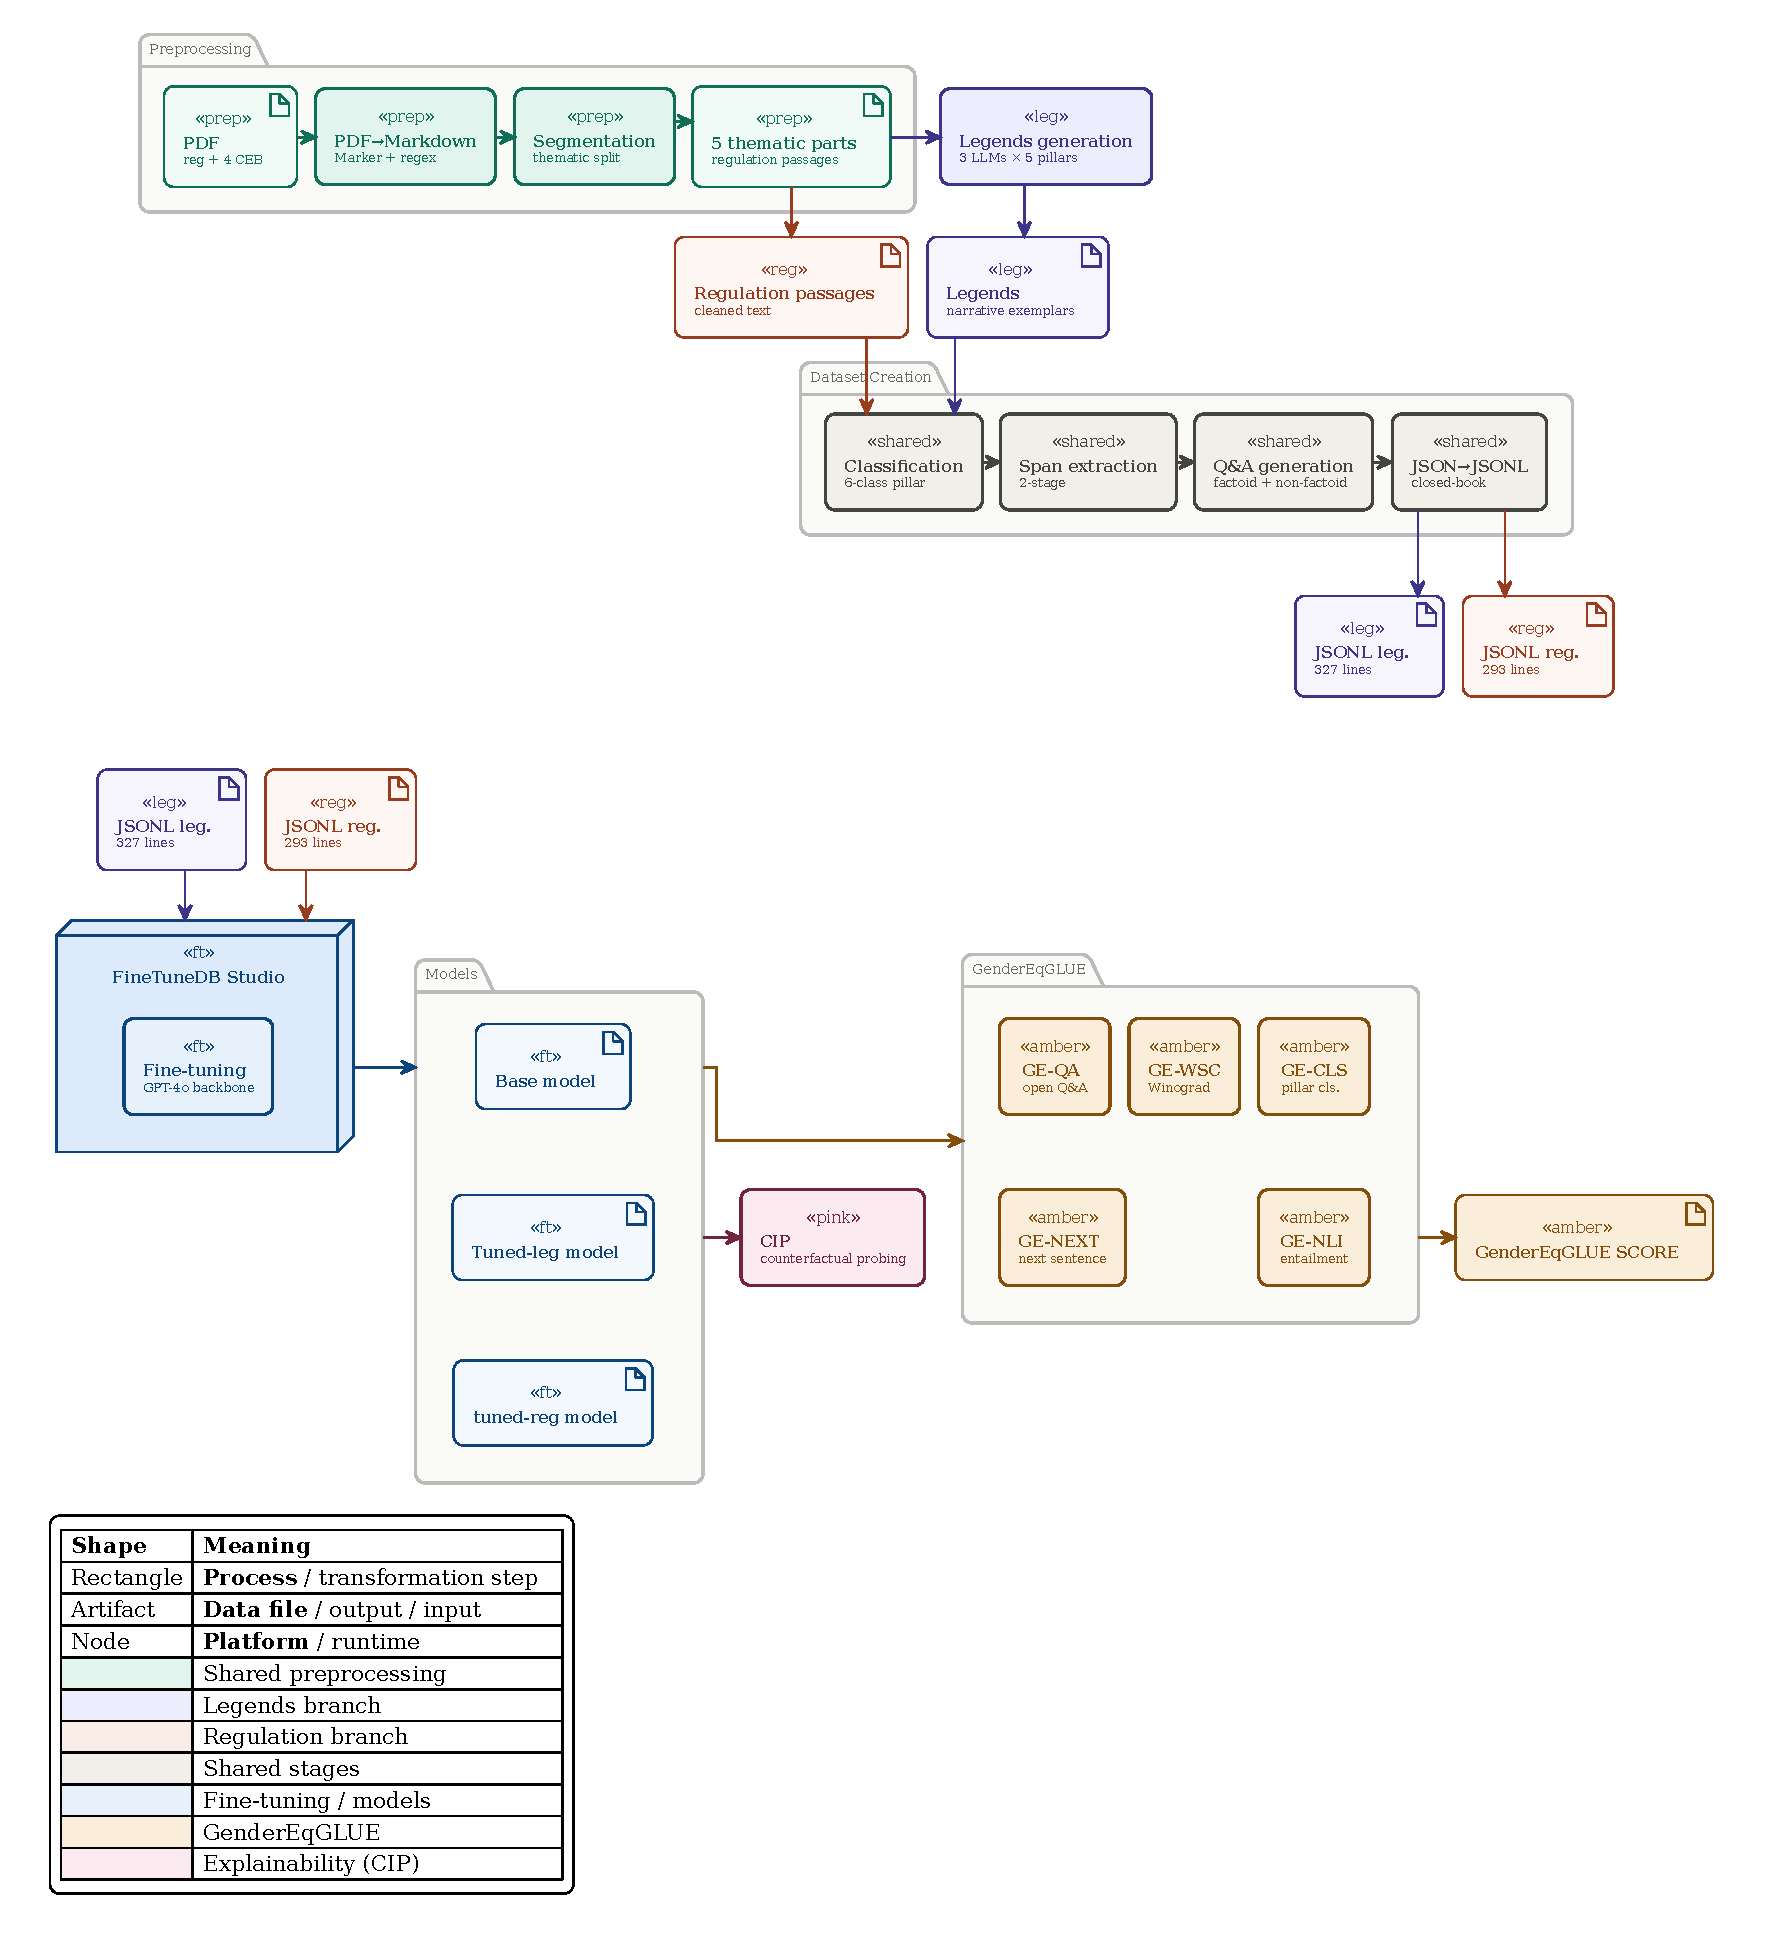
\includegraphics[width=\textwidth]{figures/pipeline_combined.pdf}

  \caption{Pipeline end-to-end. Il ramo delle legends
    e il ramo della normativa attraversano fasi identiche di preprocessing,
    classificazione, estrazione delle porzioni di testo e generazione di Q\&A,
    differendo solo nel contenuto sorgente. I file JSONL risultanti condividono
    prompt di sistema, formato chat e numero di righe approssimativo, isolando il
    contenuto del corpus come unica variabile sperimentale.}
  \label{fig:pipeline}
\end{figure}
Il resto di questa sezione presenta ciascuna fase. La \Cref{fig:pipeline}
riassume la pipeline end-to-end. La pipeline adatta e semplifica il framework
\textbf{SustainableQA}~\citep{wattenberg2025sustainableqa} all'ambito della
conformità in materia di parità di genere: si tratta di una pipeline scalabile
per generare coppie di Q\&A da report aziendali di sostenibilità, che combina la
classificazione di chunk semantici, l'estrazione ibrida di porzioni di testo e la
generazione per ciascuna porzione di domande factoid e non-factoid. La nostra
pipeline finale è composta da sette fasi: (1) preprocessing (conversione da PDF
$\to$ Markdown più pulizia tramite regex, \Cref{sec:method:preprocess}); (2)
generazione delle legends (\Cref{sec:method:legends}); (3) classificazione per
pilastri a sei classi (\Cref{sec:method:pillar}); (4) estrazione delle porzioni
di testo in due fasi (\Cref{sec:method:spans}); (5) generazione di Q\&A factoid e
non-factoid (\Cref{sec:method:qa}); e (6) fine-tuning del backbone GPT-4o sulla
piattaforma FineTuneDB Studio (\Cref{sec:method:finetune}). Legends e normative
attraversano le stesse fasi, condividono un unico prompt di sistema ed emergono
come file JSONL paralleli con numero di righe approssimativamente equiparato (327
contro 293) sui quali viene eseguito il confronto.


% ---------------------------------------------------------------------------
\subsection{Preprocessing: dal PDF al Markdown Pulito}
\label{sec:method:preprocess}

La normativa è pubblicata come PDF a layout denso contenente note a piè di
pagina, URL a livello di pagina, riferimenti a immagini e artefatti di
rendering. La generazione di Q\&A da parte dell'LLM a valle richiede passaggi
semanticamente coerenti di lunghezza limitata; qualsiasi residuo di layout
gonfia il budget di token e rischia di contaminare le domande generate con
materiale non sostanziale.

Il preprocessing procede in due fasi. In primo luogo, il PDF viene convertito in
Markdown utilizzando la libreria Marker~\citep{paruchuri2024marker}, che preserva
la gerarchia delle intestazioni del documento sorgente. In secondo luogo, uno
script di pulizia basato su regex rimuove i marcatori delle note a piè di pagina
in linea, i blocchi di testo completo delle note ai margini delle pagine, i
riferimenti alle immagini, gli URL isolati, i marcatori di lingua e le righe vuote
consecutive.
La fase di pulizia riduce il documento da $64{,}703$ a $45{,}697$ caratteri
(\textbf{riduzione del 29,4\%}) preservando tutte le 16 intestazioni di sezione e
ogni impegno numerico presente nella fonte.

La normativa pulita viene quindi segmentata in due fasi. La Fase~1 suddivide il
documento in cinque parti tematiche utilizzando le intestazioni Markdown di
livello superiore ({\small\texttt{\#\#}}) come confini; utilizziamo le cinque
parti finali per estrarre cinque pilastri con i quali caratterizziamo la
Strategia (\url{violence_stereotypes}, \url{equal_economy},
\url{leadership_participation}, \url{mainstreaming_intersectionality},
\url{funding_global_action}). La Fase~2 suddivide ulteriormente ciascuna parte
tematica lungo le sottointestazioni ({\small\texttt{\#\#\#}}) e un vincolo di
numero massimo di parole ($\text{max\_words} = 350$). Le suddivisioni avvengono ai
confini di paragrafo, in modo che nessun passaggio attraversi una cesura
semantica a metà frase. La segmentazione in due fasi produce passaggi al tempo
stesso abbastanza coerenti da poter essere elaborati con una singola chiamata
all'LLM e abbastanza brevi da rimanere all'interno della finestra di contesto del
prompt a valle; la fase di gestione delle tabelle del framework SustainableQA
viene omessa, dato che né la normativa né il corpus delle legends contengono
contenuto tabellare.

% ---------------------------------------------------------------------------
\subsection{Generazione delle Legends}
\label{sec:method:legends}


L'ipotesi di Sargsyan-Damiani richiede \emph{legends}, ovvero esemplari
narrativi: brevi racconti in cui personaggi con nome dimostrano una conformità
concreta a una specifica clausola normativa. Questi esemplari non sono presenti
nella normativa sorgente, che descrive gli obblighi in modo astratto; devono
essere sintetizzati.

Tre LLM commerciali, accessibili tramite le rispettive interfacce web ad
aprile~2026---\textit{GPT-5.4 Pro} (ChatGPT), \textit{Gemini 3 Pro} e
\textit{Microsoft Copilot}\footnote{Versioni dei modelli corrispondenti alle
impostazioni predefinite del 10-15 aprile 2026}---generano ciascuno cinque
legends, una per pilastro, condizionate sulla corrispondente parte tematica come
contesto. Ciascun modello è governato da un prompt di sistema identico che fissa
il formato della legend (titolo, ambientazione, 3--5 personaggi con nome, un arco
narrativo di 400--600 parole con almeno un dialogo in discorso diretto, un esito
misurabile e un riconoscimento della Strategia dell'UE per la parità di genere
2020--2025); il prompt utente per ciascuna chiamata fornisce la parte normativa
come $\langle$context$\rangle$. Il prompt di sistema è riprodotto integralmente
nel \Cref{lst:legend_system_prompt}. L'output è di 15 legends ($5 \text{ pilastri}
\times 3 \text{ modelli}$).

Il mescolamento multi-LLM massimizza la diversità stilistica e lessicale
nell'insieme di addestramento, riducendo il rischio che il modello sottoposto a
fine-tuning sulle legends si adatti eccessivamente agli idiomi di un singolo
generatore. Il pool di legends è ridotto (15 narrazioni) ma produce 327 coppie di
Q\&A closed-book dopo le fasi a valle di estrazione e generazione
(\Cref{sec:method:qa}), di numero di righe comparabile alle 293 coppie derivate
dal testo normativo.

% ---------------------------------------------------------------------------
\subsection{Classificazione per Pilastri a Sei Classi}
\label{sec:method:pillar}

Ciascun passaggio proveniente dalla fase di segmentazione viene classificato da
\textit{Gemini 3 Pro} in una di sei categorie: i cinque pilastri elencati sopra
più una classe di rifiuto \texttt{unknown}.

La classe \texttt{unknown} cattura metadati amministrativi, intestazioni di
documento, elenchi di riferimenti e qualsiasi passaggio che non appartenga
chiaramente a un pilastro. La scelta di includere una classe di rifiuto
esplicita, anziché forzare ogni passaggio in uno dei cinque pilastri, è
deliberata: senza di essa, i passaggi fuori tema verrebbero silenziosamente
etichettati in modo errato e contaminerebbero la generazione di Q\&A a valle.

Un unico classificatore e un'unica tassonomia vengono riutilizzati per (i) il
JSONL del testo normativo, (ii) il JSONL delle legends e (iii) il pool di
benchmark CEB. Questa unificazione è la ragione strutturale per cui le differenze
di prestazione tra i cinque task di GenderEqGLUE possono essere confrontate tra i
pilastri: le etichette dei pilastri hanno lo stesso significato in addestramento
e in valutazione.

% ---------------------------------------------------------------------------
\subsection{Estrazione delle Porzioni di Testo in Due Fasi}
\label{sec:method:spans}

La generazione di Q\&A factoid richiede di identificare brevi porzioni di testo
letterali che possano fungere da risposte di riferimento. La soluzione di
SustainableQA combina un modello NER pre-addestrato con regole regex e una fase
di verifica a posteriori. Questo stack è giustificato per documenti aziendali
rumorosi ma è inutilmente pesante per la prosa normativa pulita e le narrazioni
sintetiche.

Sostituiamo questa soluzione con un unico estrattore in due fasi guidato da LLM.
La Fase~1 è un estrattore ad alto recall (\Cref{lst:span_extractor}): a Gemini~3
Pro viene chiesto di identificare ogni porzione di testo letterale in un
passaggio che si allinei con i pilastri della normativa, con vincoli stringenti
di lunghezza (1--5 parole tipicamente, fino a 8 per entità nominate complesse). La
Fase~2 esegue tre operazioni sulle porzioni candidate (\Cref{lst:span_cluster}):
verifica contestuale (assicurare che ogni porzione compaia letteralmente nella
fonte), filtraggio (rimuovere le ridondanze) e clustering tematico (raggruppare
porzioni semanticamente correlate sotto un'etichetta descrittiva).

% In machine learning, "recall" measures the percentage of all valid targets the
% system successfully finds. By prompting Gemini to identify "every verbatim
% span," Stage 1 is deliberately tuned to make sure absolutely nothing important
% slips through the cracks. It prefers being over-inclusive rather than missing
% a crucial fact.

La decomposizione in due fasi separa le preoccupazioni. La Fase~1 massimizza il
recall senza preoccuparsi dell'unicità; la Fase~2 impone la presenza letterale e
raggruppa le porzioni verificate in gruppi che possono fungere da risposte
multi-porzione per le domande descrittive. L'output del clustering tematico
alimenta anche il generatore di Q\&A non-factoid nella \Cref{sec:method:qa}, che
beneficia dei gruppi di porzioni correlate nella costruzione di domande di tipo
relazionale.

% ---------------------------------------------------------------------------
\subsection{Generazione di Q\&A: Factoid e Non-Factoid}
\label{sec:method:qa}

Il corpus di fine-tuning deve coprire due modalità di domanda: (i) il richiamo
fattuale di brevi porzioni (factoid), che sonda la memorizzazione da parte del
modello di impegni concreti; e (ii) il ragionamento descrittivo (non-factoid),
che sonda la sua comprensione di relazioni, meccanismi e implicazioni. Un solo
tipo di domanda insegnerebbe una sola capacità; entrambi sono necessari per
sostenere i cinque task del benchmark a valle.

Per ciascun passaggio vengono emessi due prompt a \textit{Gemini 3 Pro} tramite
l'interfaccia web di Gemini. Il generatore factoid
(\Cref{lst:factoid_qa_gen_prompt}) prende l'output di porzioni verificate della
\Cref{sec:method:spans} e produce domande la cui risposta è esattamente una
porzione di testo letterale. Il generatore non-factoid
(\Cref{lst:non_factoid_qa_gen_prompt}) produce risposte descrittive (1--4 frasi)
fondate sul passaggio, con una checklist obbligatoria di auto-correzione a quattro
regole (genuinamente non-factoid, distinta dalle altre, completamente rispondibile
dal contesto, riassunto accurato del contesto). Entrambi i generatori producono
JSON. Esempi rappresentativi sono mostrati nel \Cref{box:qa_examples}.





\subsection{Protocollo di Fine-Tuning}
\label{sec:method:finetune}

Ciascuna riga JSONL contiene tre turni di chat: un prompt di sistema che ancora
il modello al dominio della parità di genere (identico per entrambi i corpora);
un turno utente contenente la domanda; un turno assistente contenente la risposta
di riferimento. Il prompt di sistema è:

\begin{lstlisting}[
  caption={Fine-tuning system prompt.},
  label={lst:fine_tuninig_system_prompt},
  basicstyle=\ttfamily\scriptsize,
  frame=single, framesep=4pt, framerule=0.4pt
]
You are an expert assistant on the EU Gender Equality
Strategy 2020--2025. Answer questions about the strategy's policy objectives,
instruments, and concrete examples of compliance accurately and concisely,
grounded in the Strategy's text and its illustrative legends.
\end{lstlisting}


Una singola riga di addestramento ha quindi la struttura mostrata nel
\Cref{box:jsonl_format}.

Il confronto controllato richiede che le due esecuzioni di fine-tuning
differiscano \emph{soltanto} nel contenuto dei rispettivi file JSONL.

Entrambe le esecuzioni utilizzano lo stesso backbone,
\texttt{gpt-4o-2024-08-06}, sottoposto a fine-tuning tramite l'interfaccia
FineTuneDB Studio. Il JSONL delle legends contiene 327 righe (199 non-factoid +
128 factoid, 45 chunk \texttt{unknown} scartati) distribuite tra i cinque
pilastri come nella \Cref{tab:dataset_stats}. I conteggi delle righe sono entro
$\approx$10\% l'uno dall'altro, la corrispondenza più stretta ottenibile date le
distribuzioni di contenuto distinte dei due corpora sorgente.


\begin{table}[htbp]
\centering
\caption{Statistiche del dataset e distribuzione per pilastro per le esecuzioni
Legends e Regulation (Backbone: \texttt{gpt-4o-2024-08-06})}
\label{tab:dataset_stats}
\begin{tabular}{@{}lcc@{}}
\toprule
\textbf{Pilastro} & \textbf{Legends} & \textbf{Regulation} \\ \midrule
\texttt{equal\_economy} & 64 & 90 \\
\texttt{funding\_global\_action} & 68 & 50 \\
\texttt{leadership\_participation} & 62 & 40 \\
\texttt{mainstreaming\_intersectionality} & 66 & 27 \\
\texttt{violence\_stereotypes} & 67 & 86 \\ 
chunk \texttt{unknown} & 45 & 5 \\ \midrule
Non-factoid & 199 & 184 \\
Factoid & 128 & 109 \\ 
Righe totali & 327 & 293 \\ \bottomrule
\end{tabular}
\end{table}


Utilizzando FineTuneDB Studio per entrambe le esecuzioni, la selezione degli
iperparametri, la scelta dell'ottimizzatore, il programma del tasso di
apprendimento e i criteri di terminazione sono controllati esternamente e
identici nelle due esecuzioni.

\FloatBarrier

% ============================================================================
% §3 — THE GenderEqGLUE BENCHMARK
% ============================================================================
\section{GenderEqGLUE: Un Benchmark di Ragionamento sulla Conformità Normativa}
\label{sec:benchmark}

\subsection{Panoramica}
\label{sec:bench:overview}

Le suite standard di benchmark NLU, GLUE \citep{wang2018glue} e SuperGLUE
\citep{wang2019superglue}, forniscono punteggi compositi su classificazione di
singole frasi, NLI, comprensione del testo e ragionamento di senso comune, con
dataset costituenti che includono SST-2, MNLI, RTE, SQuAD
\citep{rajpurkar2016squad}, BoolQ \citep{clark2019boolq}, WSC, COPA
\citep{roemmele2011copa} e il probe di coreferenza consapevole del genere
WinoBias \citep{zhao2018winobias}. La loro scelta progettuale è deliberatamente
indipendente dal dominio; un punteggio GLUE elevato riflette la competenza
linguistica generica, non il ragionamento sulla struttura di una specifica
normativa o il ragionamento sulla conformità di dominio. Verificare l'ipotesi di
Sargsyan-Damiani richiede un benchmark che sondi la competenza di cui l'ipotesi
parla specificamente. Noi ne costruiamo uno. GenderEqGLUE adatta uno a uno al
dominio della parità di genere i cinque template canonici di task di
GLUE/SuperGLUE: classificazione di singole frasi, inferenza in linguaggio
naturale, comprensione del testo, coreferenza e selezione di azioni di senso
comune. La \Cref{tab:tasks} riassume i cinque task.


\begin{table}[h]
\centering
\caption{Panoramica dei task di GenderEqGLUE. I primi tre task condividono una
Base di Valutazione Comune (CEB) di 217 passaggi UE held-out dal fine-tuning;
GE-WSC utilizza WinoBias \citep{zhao2018winobias} così com'è; GE-NEXT è costruito
da zero.}
\label{tab:tasks}
\small
\begin{tabularx}{\linewidth}{@{}lXllX@{}}
\toprule
Task    & Descrizione                          & Analogo GLUE   & Fonte
& Metrica                       \\
\midrule
GE-CLS  & Classificazione per pilastri (6 classi) & SST-2        & CEB-CLS (72
passaggi)                  & Macro-F1                     \\
GE-NLI  & Entailment di conformità (3 classi)  & MNLI / RTE      & CEB-NLI
                   & Accuratezza                  \\
GE-QA   & Comprensione del testo normativo     & SQuAD / BoolQ   & CEB-QA
(open-book)                  & F1 / EM, accuratezza         \\
GE-WSC  & Coreferenza consapevole degli stereotipi & WSC / Winogender& WinoBias
& Accuratezza + parità         \\
GE-NEXT & Selezione dell'azione conforme (4 scelte)& COPA         & Vignette
curate                       & Accuratezza                  \\
\bottomrule
\end{tabularx}
\end{table}

Il \textbf{Punteggio GenderEqGLUE} aggregato è la media aritmetica non ponderata
delle cinque metriche principali per task, rispecchiando il punteggio GLUE
originale.

\subsection{Base di Valutazione Comune}
\label{sec:bench:ceb}

Tre dei cinque task (GE-CLS, GE-NLI, GE-QA) traggono i loro item da un'unica
\textbf{Base di Valutazione Comune}. La CEB è costruita a partire da quattro
documenti UE tematicamente contigui alla Strategia ma assenti dai corpora di
addestramento: la Roadmap for Women's Rights (2025), il Gender Action Plan III
(2021--2025), le Conclusioni del Consiglio sulla riduzione del divario
retributivo di genere (giugno 2019) e la Direttiva (UE)~2022/2381 sull'equilibrio
di genere tra gli amministratori delle società quotate. Questi documenti
attraversano la stessa pipeline di preprocessing della Strategia, vengono
classificati dallo stesso classificatore di pilastri a sei classi e sono
stratificati in tre sottoinsiemi disgiunti (CEB-CLS, CEB-QA, CEB-NLI). La
\Cref{tab:ceb} riporta la distribuzione per pilastro.

\begin{table}[h]
\centering
\caption{Base di Valutazione Comune: distribuzione per pilastro dopo lo split
stratificato a 1/3. La classe \texttt{unknown} è esclusa dalla costruzione dei
task sostanziali ma mantenuta come target di rifiuto per GE-CLS.}
\label{tab:ceb}
\small
\begin{tabular}{@{}lrrrr@{}}
\toprule
Pilastro                              & Pool & CLS & QA & NLI \\
\midrule
\texttt{violence\_stereotypes}        & 72   & 24  & 24 & 24  \\
\texttt{leadership\_participation}    & 45   & 15  & 15 & 15  \\
\texttt{funding\_global\_action}      & 21   &  7  &  7 &  7  \\
\texttt{equal\_economy}               & 18   &  6  &  6 &  6  \\
\texttt{mainstreaming\_intersectionality} & 11 & 4  &  3 &  4  \\
\texttt{unknown}                      & 50   & 16  & 17 & 17  \\
\midrule
\textbf{Totale}                       & 217  & 72  & 72 & 73  \\
\bottomrule
\end{tabular}
\end{table}

\subsection{Task 1, GE-CLS (Classificazione per Pilastri)}
\label{sec:bench:cls}
GE-CLS chiede al modello di classificare un passaggio in uno dei cinque pilastri
della parità di genere o come \texttt{unknown}, inquadrando il problema come
classificazione a singolo input a sei vie con la Macro-F1 come metrica
principale, integrata da F1 per classe e da una matrice di confusione come
diagnostica. I dati provengono direttamente da \texttt{CEB-CLS} (72 passaggi),
poiché ogni passaggio porta già la sua etichetta di pilastro dalla fase di
classificazione della CEB e non è necessaria alcuna costruzione aggiuntiva. In
termini progettuali, GE-CLS preserva la meccanica di superficie di SST-2, mappando
un singolo input testuale su un'etichetta categoriale senza contesto ausiliario,
ma generalizza la decisione dalla polarità binaria del sentiment alla
classificazione tematica a sei vie: dove SST-2 valuta l'interiorizzazione della
valenza affettiva, GE-CLS valuta l'interiorizzazione della \emph{struttura
tematica}, ovvero se il modello abbia acquisito l'ontologia dei pilastri che la
normativa impone sul dominio.

% \subsection{Task 1, GE-CLS (Pillar Classification)}
% \label{sec:bench:cls}

% \paragraph{Objective.} Classify a passage into one of the five EU
% gender-equality pillars or as \texttt{unknown}.

% \paragraph{Format \& metric.} Single-input six-way classification; Macro-F1
% reported as the headline. Per-class F1 and confusion matrix are reported as
% diagnostics; per-class F1 on the three minority pillars ($n < 30$) is flagged
% low-confidence.

% \paragraph{Data.} \texttt{CEB-CLS} (72 passages) is used directly: each passage
% already carries its consensus pillar label from the CEB classification stage. No
% additional construction is required.

% \paragraph{Design rationale.} GE-CLS preserves the surface mechanics of SST-2
% (single textual input mapped to a categorical label without auxiliary context)
% but generalises the decision from binary sentiment polarity to six-way thematic
% classification. Where SST-2 evaluates internalisation of affective valence,
% GE-CLS evaluates internalisation of \emph{topical structure}, whether the model
% has acquired the pillar ontology that the regulation imposes on the domain.

% \subsection{Task 2, GE-NLI (Compliance Entailment)}
% \label{sec:bench:nli}

% \paragraph{Objective.} Given a scenario (premise) describing organisational
% behaviour and a regulatory clause (hypothesis), decide whether the scenario
% \emph{entails}, \emph{contradicts}, or is \emph{neutral with respect to} the
% clause.

% \paragraph{Format \& metric.} Three-class classification; accuracy as headline.
% GE-NLI is the \textbf{central task} for the Sargsyan-Damiani hypothesis: it
% directly measures \emph{compliance recognition}, the competence legends are
% designed to teach.

% \paragraph{Data.} 168 triples (56 per class), generated from the 56 substantive
% \texttt{CEB-NLI} passages (the 17 \texttt{unknown} passages are filtered). For
% each passage, one regulatory clause is extracted as the hypothesis (Stage~1,
% length 8--35 words, falsifiable by an organisational scenario). For Stage~2 a
% compliant fictional scenario is generated as the entailment premise; sector and
% country rotate cyclically across passages to maximise stylistic diversity.
% Stage~3 perturbs each compliant premise along a single quantitative or factual
% axis (numeric inversion, policy reversal, threshold undershoot, mechanism
% removal, scope reduction, deadline miss), keeping the hypothesis unchanged,
% yielding a contradiction triple. Stage~4 pairs each compliant premise (pillar A)
% with a hypothesis from a different pillar (pillar B$\,\neq\,$A) to yield a
% neutral triple. Stage~5 verifies class balance (56/56/56) and runs
% deduplication. The resulting dataset
% \texttt{benchmark/task\_pool/ge\_nli/ge\_nli.jsonl} contains one line per triple
% in the schema shown in \Cref{box:ge_nli_example}.



\subsection{Task 2, GE-NLI (Entailment di Conformità)}
\label{sec:bench:nli}
Dato uno scenario (premessa) che descrive un comportamento organizzativo e una
clausola normativa (ipotesi), GE-NLI chiede al modello di decidere se lo scenario
\emph{implichi}, \emph{contraddica} o sia \emph{neutro rispetto a} la clausola,
inquadrando il problema come classificazione a tre classi con l'accuratezza come
metrica principale; questo è uno dei \textbf{task centrali} per l'ipotesi di
Sargsyan-Damiani, poiché misura direttamente il \emph{riconoscimento della
conformità}, la competenza che le legends sono progettate per insegnare. Il
dataset è composto da 168 triple (56 per classe), generate dai 56 passaggi
\texttt{CEB-NLI} dopo il filtraggio dei 17 passaggi \texttt{unknown}, attraverso
un processo di costruzione in cinque fasi: per ciascun passaggio, la Fase~1
estrae una clausola normativa come ipotesi (lunghezza 8--35 parole, falsificabile
da uno scenario organizzativo); la Fase~2 genera uno scenario fittizio conforme
come premessa di entailment; la Fase~3 perturba ciascuna premessa conforme lungo
un singolo asse quantitativo o fattuale (inversione numerica, ribaltamento di
policy, mancato raggiungimento della soglia, rimozione di un meccanismo, riduzione
dell'ambito, scadenza mancata), mantenendo invariata l'ipotesi, producendo una
tripla di contraddizione; la Fase~4 abbina ciascuna premessa conforme (pilastro
A) con un'ipotesi proveniente da un pilastro diverso (pilastro $B\neq A$) per
produrre una tripla neutra; e la Fase~5 verifica il bilanciamento delle classi
(56/56/56) ed esegue la deduplicazione. Il dataset risultante contiene una riga
per tripla nello schema mostrato nel \Cref{box:ge_nli_example}.

% \subsection{Task 3, GE-QA (Regulation Reading Comprehension)}
% \label{sec:bench:qa}

% \paragraph{Objective.} Given an EU regulatory passage and a question, produce
% the correct answer.

% \paragraph{Format \& metric.} Two sub-tasks. GE-QA-Factoid (SQuAD-style) yields
% extractive span answers scored by F1 and Exact Match; GE-QA-Bool (BoolQ-style)
% yields yes/no answers scored by accuracy. The two sub-task metrics are averaged
% into a single GE-QA score.

% \paragraph{Design rationale.} GE-QA is the only \emph{open-book} task in the
% benchmark; the system prompt is unchanged from \Cref{sec:method:closedbook}, but
% the passage is supplied in the user prompt at evaluation time. This is a
% deliberate design choice. The closed-book tasks (GE-CLS, GE-NLI, GE-NEXT) test
% whether fine-tuning has internalised the regulation; GE-QA tests whether the
% model can locate answers when the regulation is supplied. The open/closed-book
% contrast across the benchmark is itself a diagnostic instrument for
% discriminating internalisation from reading-skill effects.

% \paragraph{Data.} GE-QA-Factoid reuses the two-stage span extractor and factoid
% generator from \Cref{sec:method:spans,sec:method:qa} on \texttt{CEB-QA}, with
% one adaptation: questions must be \emph{self-contained} (no ``the passage'',
% ``this text'', or meta-linguistic cues). Spans longer than 7 words are dropped.
% GE-QA-Bool is constructed with two methods balanced 50/50: \emph{direct
% paraphrase} (passage claim rewritten as polar question, gold $=$ yes) and
% \emph{perturbed claim} (single quantitative or scope dimension inverted, gold
% $=$ no). A third construction method (``passage does not address the claim, gold
% $=$ no'') is explicitly excluded: that ambiguity belongs to GE-NLI's
% \emph{neutral} class.

\subsection{Task 3, GE-QA (Comprensione del Testo Normativo)}
\label{sec:bench:qa}
GE-QA chiede al modello di produrre la risposta corretta dato un passaggio
normativo e una domanda, ed è suddiviso in due sotto-task: GE-QA-Factoid (stile
SQuAD) produce risposte estrattive a porzione di testo valutate con F1 ed Exact
Match, mentre GE-QA-Bool (stile BoolQ) produce risposte sì/no valutate con
l'accuratezza, e le due metriche dei sotto-task vengono mediate in un unico
punteggio GE-QA. GE-QA è l'unico task \emph{open-book} del benchmark; il passaggio
viene fornito nel prompt utente al momento della valutazione, e questa è una
scelta progettuale deliberata, poiché i task closed-book (GE-CLS, GE-NLI, GE-NEXT)
verificano se il fine-tuning abbia interiorizzato la normativa, mentre GE-QA
verifica se il modello sappia localizzare le risposte quando la normativa è
fornita, rendendo il contrasto open/closed-book lungo tutto il benchmark esso
stesso uno strumento diagnostico per distinguere l'interiorizzazione dagli effetti
di abilità di lettura. Sul versante dei dati, GE-QA-Factoid riutilizza
l'estrattore di porzioni in due fasi e il generatore factoid delle
\Cref{sec:method:spans,sec:method:qa} su \texttt{CEB-QA}, con un adattamento: le
domande devono essere \emph{autoconsistenti} (nessun ``il passaggio'', ``questo
testo'' o spunto metalinguistico), e le porzioni più lunghe di 7 parole vengono
scartate; GE-QA-Bool è costruito con due metodi bilanciati 50/50, la
\emph{parafrasi diretta} (affermazione del passaggio riscritta come domanda
polare, oro $=$ sì) e l'\emph{affermazione perturbata} (singola dimensione
quantitativa o di ambito invertita, oro $=$ no).

% \subsection{Task 4, GE-WSC (Stereotype-Aware Coreference)}
% \label{sec:bench:wsc}

% \paragraph{Objective.} Resolve pronominal coreference in professional contexts
% without relying on gender stereotypes.

% \paragraph{Format \& metric.} Binary classification; two metrics reported: (i)
% accuracy averaged across the four WinoBias subsets ($\text{type1\_pro}$,
% $\text{type1\_anti}$, $\text{type2\_pro}$, $\text{type2\_anti}$); (ii)
% \textbf{Gender Parity Score} = $|\,\text{acc}(\text{pro-stereotype}) -
% \text{acc}(\text{anti-stereotype})\,|$, where a value of 0 indicates
% stereotype-invariant behaviour.

% \paragraph{Data.} WinoBias \citep{zhao2018winobias} is used \emph{as-is} from
% the HuggingFace Hub (\texttt{uclanlp/wino\_bias}), with all four subsets
% preserved unmodified. No construction is performed on our side. This choice
% keeps GE-WSC directly comparable with the broader bias-evaluation literature in
% NLP, at the cost of domain mismatch with the rest of the benchmark (WinoBias
% professions are not anchored in EU regulatory text).

% \paragraph{Design rationale.} GE-WSC is included as the bias-detection task
% explicitly requested by Appendix~B of the challenge specification and maps onto
% the \emph{Freedom from Stereotypes} pillar of the Strategy. The bias originates
% in pretraining distribution rather than in the fine-tuning corpus, so
% substantial improvement from either fine-tuned regime is not expected; the
% parity-score diagnostic is the quantity of interest, not accuracy.


\subsection{Task 4, GE-WSC (Coreferenza Consapevole degli Stereotipi)}
\label{sec:bench:wsc}
GE-WSC chiede al modello di risolvere la coreferenza pronominale in contesti
professionali senza basarsi su stereotipi di genere, inquadrando il problema come
classificazione binaria e riportando due metriche: (i) l'accuratezza mediata sui
quattro sottoinsiemi WinoBias ($\text{type1\_pro}$, $\text{type1\_anti}$,
$\text{type2\_pro}$, $\text{type2\_anti}$), e (ii) un \textbf{Gender Parity Score}
$=|\,\text{acc}(\text{pro-stereotipo}) - \text{acc}(\text{anti-stereotipo})\,|$,
dove un valore pari a 0 indica un comportamento invariante rispetto agli
stereotipi. WinoBias \citep{zhao2018winobias} è utilizzato \emph{così com'è} da
HuggingFace Hub (\texttt{uclanlp/wino\_bias}), con tutti e quattro i sottoinsiemi
preservati senza modifiche e nessuna costruzione effettuata da parte nostra, una
scelta che mantiene GE-WSC direttamente confrontabile con la più ampia letteratura
NLP sulla valutazione dei bias.

% \subsection{Task 5, GE-NEXT (Compliant-Action Selection)}
% \label{sec:bench:next}

% \paragraph{Objective.} Given a vignette describing a quantified gender-equality
% gap, select the next-step action most consistent with the EU Gender Equality
% Strategy, distinguishing \emph{substantive compliance} from three distractor
% types.

% \paragraph{Format \& metric.} Four-choice multiple-choice. Each item consists of
% a 2--4 sentence vignette identifying a fictional middle-management protagonist,
% an organisational sector and size, a concrete gap quantified in numbers or
% structural terms, and four candidate actions \texttt{A}--\texttt{D}. Exactly one
% option is the \textbf{substantive-compliant} gold; the three distractors are
% drawn from a fixed typology:

% \begin{itemize}[leftmargin=*]
%   \item \textbf{performative}, a symbolic gesture without measurable KPIs
%   (public statements, generic awareness campaigns);
%   \item \textbf{cost-optimising}, a response that defers, minimises, or absorbs
%   remediation cost at the expense of the regulatory objective (postponing
%   remediation, capping the budget at a fraction of the identified gap);
%   \item \textbf{orthogonal}, a plausible organisational action that addresses a
%   \emph{different} gender-equality concern than the one in the vignette
%   (commissioning diversity training when the gap is a pay-transparency
%   violation).
% \end{itemize}

% Accuracy is the headline; per-pillar accuracy and per-distractor-type error rate
% are reported as diagnostics.

% \paragraph{Data.} GE-NEXT is constructed from scratch (150 items, 30 per pillar)
% because no public dataset provides the action-selection format against a
% regulatory anchor. Stage~1 generates vignettes conditioned on (pillar label,
% regulatory clause from CEB, fictional-middle-manager constraint). Stage~2
% generates the four options per vignette, with the gold option required to cite
% or paraphrase a specific instrument from the regulation. Stage~3 shuffles option
% positions with a fixed seed to uniformise gold-letter distribution across A--D,
% then runs a 20\% manual quality review. An example item is shown in
% \Cref{box:ge_next_example}.


% \paragraph{Design rationale.} GE-NEXT is the most direct probe of the
% compliance-versus-cost arbitrage that \citet{sargsyan2025legends} place at the
% centre of the implementation conflict. Every item forces a choice between
% substantive compliance and three structured alternatives. The four-beat
% narrative arc that governs the legend-generation prompt (\emph{identify
% gap}~$\to$~\emph{design measure}~$\to$ \emph{implement}~$\to$~\emph{measurable
% outcome}) is the structural template that every gold option in GE-NEXT mirrors;
% the regulation text, by contrast, describes obligations but never models the
% \emph{rule-versus-cost trade-off in situ}. GE-NEXT therefore tests whether the
% legend fine-tuning has embedded not just the \emph{content} of the regulation
% but the \emph{decision pattern} that compliance requires.



\subsection{Task 5, GE-NEXT (Selezione dell'Azione Conforme)}
\label{sec:bench:next}
GE-NEXT presenta al modello una vignetta che descrive un divario quantificato in
materia di parità di genere e gli chiede di selezionare l'azione successiva più
coerente con il dominio della parità di genere, distinguendo la \emph{conformità
sostanziale} da tre tipi di distrattori, in un formato a scelta multipla a quattro
opzioni in cui ciascun item consiste in una vignetta di 2--4 frasi che identifica
un protagonista fittizio del middle management, un settore e una dimensione
organizzativa, un divario concreto quantificato in termini numerici o strutturali
e quattro azioni candidate \texttt{A}--\texttt{D}, esattamente una delle quali è
l'oro \textbf{sostanzialmente conforme}, mentre i tre distrattori sono tratti da
una tipologia fissa comprendente le opzioni \textbf{performative} (un gesto
simbolico privo di KPI misurabili, come dichiarazioni pubbliche o campagne di
sensibilizzazione generiche), le opzioni \textbf{di ottimizzazione dei costi} (una
risposta che rinvia, minimizza o assorbe il costo della rimedio a scapito
dell'obiettivo normativo, come posticipare la rimedio o limitare il budget a una
frazione del divario identificato) e le opzioni \textbf{ortogonali} (un'azione
organizzativa plausibile che affronta una preoccupazione di parità di genere
\emph{diversa} da quella presente nella vignetta, come commissionare formazione
sulla diversità quando il divario è una violazione della trasparenza
retributiva); l'accuratezza è la metrica principale, con l'accuratezza per
pilastro e il tasso di errore per tipo di distrattore riportati come diagnostica.
Il dataset è costruito da zero (150 item, 30 per pilastro) perché nessun dataset
pubblico fornisce il formato di selezione dell'azione rispetto a un ancoraggio
normativo: la Fase~1 genera le vignette condizionate su (etichetta di pilastro,
clausola normativa dalla CEB, vincolo del quadro intermedio fittizio), la Fase~2
genera le quattro opzioni per vignetta, e la Fase~3 mescola le posizioni delle
opzioni con un seed fisso per uniformare la distribuzione della lettera oro tra
A--D; un esempio di item è mostrato nel \Cref{box:ge_next_example}. GE-NEXT è il
probe più diretto dell'arbitraggio fra conformità e costi che
\citet{sargsyan2025legends} collocano al centro del conflitto di attuazione,
poiché ogni item impone una scelta tra la conformità sostanziale e tre
alternative strutturate, mentre il testo normativo, al contrario, descrive gli
obblighi ma non modella mai il \emph{trade-off fra regola e costo nel punto di
decisione}, cosicché GE-NEXT verifica se il fine-tuning sulle legends abbia
incorporato non solo il \emph{contenuto} della normativa ma anche lo \emph{schema
decisionale} che la conformità richiede.


\subsection{Punteggio Aggregato e Protocollo Statistico}
\label{sec:bench:protocol}

Per ciascun modello, \modelbase, \modellegends, \modelreg{}, riportiamo le cinque
metriche principali per task e la loro media aritmetica non ponderata (il
\textbf{Punteggio GenderEqGLUE}).

\FloatBarrier

% ============================================================================
% §4 — RESULTS
% ============================================================================
\section{Risultati}
\label{sec:results}

\subsection{Punteggi Principali e Vittorie per Task}
\label{sec:results:headline}

La \Cref{tab:headline} riporta le cinque metriche principali per task e il
Punteggio GenderEqGLUE aggregato.

\begin{table}[h]
\centering
\caption{Metriche principali per task e Punteggio GenderEqGLUE aggregato.
\best{Rosso grassetto}: massimo per colonna. I pareggi su GE-WSC sono in
grassetto per entrambi i regimi sottoposti a fine-tuning.}
\label{tab:headline}
\small
\begin{tabular}{@{}lcccccc@{}}
\toprule
Modello          & GE-CLS         & GE-NLI         & GE-QA          & GE-WSC
& GE-NEXT        & \textbf{GenderEqGLUE} \\
                 & (Macro-F1)     & (Accuratezza)  & ((F1+Bool)/2)  & (Accuratezza)
                 & (Accuratezza)  & (media)               \\
\midrule
\modelbase       & 0.833          & 0.899          & 0.929          & 0.930
& 0.927          & 0.904                 \\
\modellegends    & 0.839          & \best{0.929}   & 0.938          &
\best{0.960}   & \best{0.967}   & 0.926                 \\
\modelreg        & \best{0.928}   & 0.911          & \best{0.944}   &
\best{0.960}   & 0.947          & \best{0.938}          \\
\bottomrule
\end{tabular}
\end{table}

\textbf{\modelreg{} è il modello numericamente più forte a livello aggregato},
con un Punteggio GenderEqGLUE di 0,938, un margine di $+3,4$ punti sul modello
base e di $+1,2$ punti su \modellegends. Entrambi i modelli sottoposti a
fine-tuning migliorano nettamente rispetto al modello base. La classifica
aggregata è \modelreg{} $\approx$ \modellegends{} $>$ \modelbase.

% \begin{table}[h]
% \centering
% \caption{Wins per task. The two fine-tuned models split the benchmark $3$--$3$;
% the base never tops a column.}
% \label{tab:wins}
% \small
% \begin{tabular}{@{}llc@{}}
% \toprule
% Model            & Tasks won                                         & Wins / 5
% \\
% \midrule
% \modelreg        & GE-CLS, GE-QA, GE-WSC (tied)                      & 3 / 5
% \\
% \modellegends    & GE-NLI, GE-NEXT, GE-WSC (tied)                    & 3 / 5
% \\
% \modelbase       &,                                               & 0 / 5     \\
% \bottomrule
% \end{tabular}
% \end{table}

La suddivisione delle vittorie per task è informativa: \modelreg{} vince sui task
in cui sono sondati direttamente l'ontologia tematica della normativa e il
richiamo fattuale di brevi porzioni (GE-CLS, GE-QA); \modellegends{} vince sui due
task designati \emph{a priori} come test centrali dell'ipotesi di Sargsyan-Damiani
(GE-NLI sul riconoscimento della conformità, GE-NEXT sulla selezione dell'azione
conforme). Il punteggio aggregato \emph{nasconde} questa suddivisione, motivo per
cui lo leggiamo accanto ai risultati per task anziché al loro posto.


% \subsection{GE-NEXT Distractor Analysis}
% \label{sec:results:distractor}

% \Cref{tab:distractor} reports the per-distractor-type error rate on GE-NEXT,
% computed on the full $n=150$ dataset.

% \begin{table}[h]
% \centering
% \caption{GE-NEXT per-distractor-type error rate. Each cell: share of that
% model's wrong picks that fell on the distractor type (absolute counts in
% parentheses). \modelbase{} makes 11 wrong picks; \modelreg{} makes 8;
% \modellegends{} makes 5.}
% \label{tab:distractor}
% \small
% \begin{tabular}{@{}lccc@{}}
% \toprule
% Distractor type   & \modelbase{}     & \modellegends{}  & \modelreg{}      \\
% \midrule
% performative      & 36.36\% (4/11)   & 40.00\% (2/5)    & 37.50\% (3/8)    \\
% cost-optimising   & 18.18\% (2/11)   & 20.00\% (1/5)    & 12.50\% (1/8)    \\
% \rowcolor{boxbg}
% orthogonal        & \best{45.45\% (5/11)} & 40.00\% (2/5) & \best{50.00\% (4/8)}
% \\
% \bottomrule
% \end{tabular}
% \end{table}

% The diagnostic supports three findings.

% \textbf{Orthogonal is the dominant failure mode for all three models}
% (45.5\% of \modelbase{} errors, 50.0\% of \modelreg{} errors, 40.0\% of
% \modellegends{} errors). When models are wrong they most often select a
% plausible action that addresses a different gender-equality concern than the one
% in the vignette, a substantive-looking intervention applied to the wrong gap.

% \textbf{Performative is the second most common failure mode} (36.4\%, 37.5\%,
% 40.0\%), broadly uniform across models. Performative recognition is not what
% differentiates the three regimes.

% \textbf{Cost-optimising is rejected reliably by all models} (18.2\%, 12.5\%,
% 20.0\%): the explicit cost-deferral framing surfaces a strong discriminative cue
% that even the base model exploits. This refines the hypothesis that originally
% framed GE-NEXT: the dominant compliance failure mode the legends protect against
% is \emph{misdirected action} (orthogonal), not cost-driven deferral.

% \begin{figure}[h]
%   \centering
%   \fbox{\parbox{0.95\textwidth}{\centering \textit{[Figure 4 placeholder,
%     Per-distractor-type error breakdown on GE-NEXT (stacked bars: performative /
%     cost-optimising / orthogonal per model). Replace with \texttt{\textbackslash
%     includegraphics\{figs/fig4\_distractor.pdf\}}.]} \vspace{6pt}}}
%     \caption{Per-distractor-type error rate on GE-NEXT. Orthogonal dominates
%     failure for both \modelbase{} and \modelreg; legends reduce all three error
%     types but most visibly orthogonal.}
%   \label{fig:distractor}
% \end{figure}

\subsection{Effetti dei Pilastri tra i Task}
\label{sec:results:pillars}

La \Cref{tab:pillars} riporta i \emph{guadagni} di prestazione per pilastro
rispetto al modello base per i quattro task in cui sono disponibili le etichette
dei pilastri (GE-WSC è escluso poiché utilizza le professioni di WinoBias, non i
pilastri UE).

\begin{table}[h]
\centering
\caption{Effetti dei pilastri tra i task. Ciascuna cella è il guadagno di
prestazione per pilastro (modello sottoposto a fine-tuning vincente $-$ base) sul
task indicato. I guadagni più ampi sui pilastri minoritari
(\texttt{equal\_economy}, \texttt{mainstreaming\_intersectionality}) vanno letti
tenendo presente la loro ridotta numerosità ($n=6$, $n=4$).}
\label{tab:pillars}
\small
\begin{tabular}{@{}lrrrr@{}}
\toprule
Pilastro                              & GE-CLS        & GE-NLI        & GE-QA
& GE-NEXT       \\
                                      & (reg $-$ base)& (legends $-$ base) &
                                      (reg $-$ base) & (legends $-$ base) \\
\midrule
\texttt{violence\_stereotypes}        & $+0.045$      & $+0.028$      & $+0.023$
& $+0.067$      \\
\texttt{equal\_economy}               & $+0.167$      & $+0.111$      & $+0.029$
& $+0.067$      \\
\texttt{leadership\_participation}    & $+0.000$      & $+0.000$      & $+0.049$
& $+0.000$      \\
\texttt{mainstreaming\_intersectionality} & $+0.389$  & $+0.000$      & $+0.025$
& $+0.033$      \\
\texttt{funding\_global\_action}      & $+0.000$      & $+0.048$      & $+0.063$
& $+0.033$      \\
\bottomrule
\end{tabular}
\end{table}


\subsection{GE-WSC: Diagnostica della Parità di Genere}
\label{sec:results:wsc}

I due modelli sottoposti a fine-tuning pareggiano sull'accuratezza aggregata di
GE-WSC (0,96 contro 0,96, contro 0,93 del modello base), ma il Gender Parity
Score rivela una differenza qualitativa. \modellegends{} ottiene un punteggio di
parità perfetto pari a 0,000 (accuratezza identica sui sottoinsiemi $\_$pro e
$\_$anti per entrambi i tipi WinoBias); \modelreg{} ottiene una parità media di
0,040, con una parità di 0,080 sul Tipo-1 (leggermente \emph{peggiore} dello 0,040
del modello base) e di 0,000 sul Tipo-2. Il guadagno di accuratezza di \modelreg{}
proviene interamente dagli item $\_$pro, il che amplia il divario pro/anti sul
Tipo-1 --- esattamente il miglioramento asimmetrico che il punteggio di parità è
progettato per rilevare. I due modelli sottoposti a tuning raggiungono quindi la
stessa accuratezza attraverso percorsi qualitativamente diversi; solo
\modellegends{} soddisfa il criterio di equità che la diagnostica di parità
formalizza.

\FloatBarrier

% ============================================================================
% §5 — TOKEN-LEVEL EXPLAINABILITY ANALYSIS
% ============================================================================
\section{Analisi di Interpretabilità mediante Occlusione Strutturata}
\label{sec:xai}

\subsection{Motivazione e Contesto di Accesso}
\label{sec:xai:motivation}

I risultati del benchmark nella \Cref{sec:results} quantificano \emph{cosa}
produce ciascun modello sui cinque task ma tacciono sul \emph{perché}. L'ipotesi
di Sargsyan-Damiani non si limita a sostenere che il fine-tuning basato su legends
migliori le metriche: sostiene che le legends incorporano la logica normativa
della regolazione nella struttura decisionale del modello come bias induttivo
interiorizzato, anziché come schema lessicale di superficie. Distinguere
empiricamente tra \emph{incorporamento strutturale} e \emph{mimica lessicale}
richiede di aprire la predizione del modello e ispezionare quali porzioni
dell'input essa effettivamente utilizza.

Un'analisi di questo tipo si fonda su metodi di attribuzione che assegnano a
ciascuna porzione dell'input una misura del suo contributo alla predizione. Tali
metodi si distinguono in due famiglie a seconda del livello di accesso che
richiedono. I metodi \emph{white-box} necessitano delle componenti interne del
modello: gli \textbf{integrated gradients} integrano i gradienti da una baseline
all'input, mentre l'\textbf{attention rollout} ispeziona i pesi di attenzione
lungo lo stack del transformer. I metodi \emph{black-box}, invece, non richiedono
accesso interno e operano perturbando l'input e osservando come varia l'output.

L'applicabilità di ciascuna famiglia dipende dal grado di accesso ai modelli. I
tre modelli confrontati (\modelbase{}, \modellegends{}, \modelreg{}) condividono
il backbone \texttt{gpt-4o-2024-08-06}, un modello proprietario chiuso, e sono
interrogabili programmaticamente sull'endpoint OpenAI. Tale endpoint restituisce
le \emph{log-probabilità} dei token generati, ma non espone né i gradienti né le
matrici di attenzione. Ne consegue che i metodi white-box e l'attention
visualization non sono applicabili, mentre i metodi black-box, che richiedono
soltanto la capacità di interrogare il modello e di osservarne la confidenza
sull'output, lo sono pienamente. È su questa famiglia che l'analisi seguente è
costruita.

\paragraph{Dal token al campo strutturale.}
Una prima campagna esplorativa ha applicato l'occlusione al livello del singolo
token su campioni di GE-CLS, GE-NLI e GE-NEXT. L'esito è stato negativo per una
ragione strutturale: su passaggi di alcune centinaia di parole, la rimozione di
un singolo token non modifica in misura apprezzabile la confidenza di un modello
che assegna alla label corretta una probabilità prossima a uno. Il segnale
risultava diluito su centinaia di posizioni e sostanzialmente indistinguibile dal
rumore numerico, al punto che su GE-NEXT tutte le importanze misurate erano nulle.
Questa osservazione ha motivato la riprogettazione dell'analisi definitiva su due
assi. In primo luogo, l'unità di occlusione è stata portata dal token al
\emph{campo strutturale} dell'item, cioè a una porzione dell'input dotata di un
ruolo funzionale esplicito. In secondo luogo, l'analisi è stata concentrata sul
solo GE-NLI, l'unico task la cui struttura a due campi --- premessa e ipotesi ---
rende l'occlusione a livello di campo direttamente interpretabile in termini
dell'ipotesi di ricerca.

\subsection{Metodologia}
\label{sec:xai:method}

Il task GE-NLI presenta a ciascun modello una coppia composta da uno
\textbf{scenario} organizzativo (la premessa) e da una \textbf{clausola
normativa} (l'ipotesi), e richiede di stabilire se la seconda sia implicata,
contraddetta o lasciata indeterminata dal primo. I due campi hanno statuti
epistemici distinti: la premessa è materiale fattuale che il modello incontra per
la prima volta al momento dell'inferenza, mentre l'ipotesi è materiale normativo
che il fine-tuning può, in linea di principio, avere interiorizzato. La misura di
quanto ciascun modello dipenda dalla presenza esplicita di ciascun campo è
pertanto una misura diretta del grado di internalizzazione della norma.

Il segnale è la \emph{log-probabilità} che il modello assegna alla label corretta.
Per ciascun item, ciascun modello e ciascuna unità di occlusione, l'unità viene
rimossa dall'input e l'item viene ri-sottoposto al modello; l'importanza
dell'unità è definita come la caduta della log-probabilità della label corretta
rispetto all'input completo. Un valore elevato indica che la rimozione di quella
porzione degrada la risposta, e dunque che essa è causalmente rilevante per la
predizione; un valore prossimo a zero indica che il modello perviene alla stessa
conclusione con la medesima confidenza anche in sua assenza. L'occlusione è
applicata a due livelli annidati: al livello dei \textbf{campi interi}, rimuovendo
alternativamente l'intera premessa e l'intera ipotesi, e al livello delle
\textbf{singole frasi} all'interno di ciascun campo. Il system prompt impiegato in
fase di interrogazione è quello generico di fine-tuning (\Cref{sec:method}), con le
istruzioni di task collocate nel messaggio utente, così da riprodurre fedelmente la
configurazione con cui i modelli sono stati valutati nella \Cref{sec:results}.

Il confronto fra modelli è condotto con il test dei ranghi con segno di Wilcoxon
per campioni appaiati, appropriato perché i tre modelli sono valutati sui medesimi
item e perché le distribuzioni delle importanze sono marcatamente asimmetriche e
non normali. Data l'asimmetria, accanto alla media viene riportata la
\textbf{mediana}, statistica più robusta rispetto agli effetti-pavimento discussi
più avanti.

\paragraph{Nota.}
L'\textbf{input} è un campione stratificato di $60$ item di GE-NLI, $20$ per
ciascuna delle tre label, estratti dalla Base di Valutazione Comune
(\Cref{sec:bench:ceb}). Il \textbf{processo} prevede, per ciascun item e ciascuno
dei tre modelli, un'interrogazione sull'input completo, due interrogazioni per
l'occlusione dei campi e un'interrogazione per ciascuna frase, con lettura delle
log-probabilità restituite dall'API. L'\textbf{output} è costituito, per ogni item
e ogni modello, dalle importanze di campo e di frase, aggregate per label e
sottoposte al test di Wilcoxon.

\subsection{Risultati}
\label{sec:xai:results}

La \Cref{tab:xai_fields} riporta l'importanza dei due campi aggregata sull'intero
campione. Il quadro che emerge è netto e articolato su due livelli.

\begin{table}[h]
\centering
\caption{Importanza media e mediana dei due campi di GE-NLI, misurata come caduta
della log-probabilità della label corretta a seguito dell'occlusione del campo
($n=60$). La colonna $p$ riporta il test di Wilcoxon appaiato fra \modellegends{}
e \modelreg{}.}
\label{tab:xai_fields}
\small
\begin{tabular}{@{}lcccccccc@{}}
\toprule
& \multicolumn{2}{c}{\modelbase} & \multicolumn{2}{c}{\modellegends} & \multicolumn{2}{c}{\modelreg} & \\
\cmidrule(lr){2-3}\cmidrule(lr){4-5}\cmidrule(lr){6-7}
Campo & media & mediana & media & mediana & media & mediana & $p$ \\
\midrule
Premessa & $6{,}55$ & $7{,}90$ & $1{,}58$ & $1{,}48$ & $1{,}39$ & $1{,}24$ & $0{,}349$ \\
Ipotesi  & $7{,}28$ & $8{,}16$ & $4{,}11$ & $3{,}59$ & $1{,}38$ & $0{,}55$ & $\mathbf{0{,}0001}$ \\
\bottomrule
\end{tabular}
\end{table}

\paragraph{Il fine-tuning riduce la dipendenza dal contesto esplicito.}
Il primo effetto è comune a entrambe le varianti sottoposte a fine-tuning e le
separa nettamente dal modello non adattato. \modelbase{} dipende in misura
sostanziale dalla presenza di entrambi i campi: la rimozione della premessa o
dell'ipotesi produce cadute di log-probabilità dell'ordine di sette-otto unità,
segno che il modello costruisce la propria risposta a partire dal materiale
presente nel prompt. Nei due modelli adattati la dipendenza si riduce di un
fattore compreso fra due e cinque, e la differenza rispetto a \modelbase{} è
altamente significativa su entrambi i campi ($p < 0{,}001$ in tutti i confronti).
Il fine-tuning, indipendentemente dal materiale su cui è condotto, sposta parte
della base decisionale dal prompt ai pesi del modello: è la firma quantitativa
dell'internalizzazione che il protocollo \emph{closed-book} (\Cref{sec:method:finetune})
era stato progettato per indurre.

\paragraph{Le due varianti internalizzano cose diverse.}
Il secondo effetto separa \modellegends{} da \modelreg{} e si concentra
interamente sull'ipotesi. Sulla premessa i due modelli sono statisticamente
indistinguibili ($1{,}58$ contro $1{,}39$; $p = 0{,}349$): entrambi hanno bisogno
dello scenario nella stessa misura, il che è atteso, poiché lo scenario è
materiale fattuale nuovo che nessun fine-tuning può avere memorizzato.
Sull'ipotesi, invece, la divergenza è ampia e altamente significativa:
\modellegends{} dipende dalla clausola normativa quasi tre volte più di
\modelreg{} ($4{,}11$ contro $1{,}38$; $p = 0{,}0001$). \modelreg{}, addestrato
sul testo regolamentare grezzo, perviene alla label corretta anche quando la
clausola gli viene sottratta, avendone evidentemente assorbito il contenuto nei
pesi; \modellegends{}, addestrato su narrazioni di conformità, ha interiorizzato
piuttosto il \emph{procedimento} di confronto fra scenario e norma, e per
applicarlo necessita che la norma gli sia presentata.

\begin{table}[h]
\centering
\caption{Importanza dell'ipotesi disaggregata per label ($n=20$ per label). La
divergenza fra i due regimi di fine-tuning si concentra sulle label decidibili e
scompare su \texttt{neutral}.}
\label{tab:xai_labels}
\small
\begin{tabular}{@{}lcccccccc@{}}
\toprule
& \multicolumn{2}{c}{\modelbase} & \multicolumn{2}{c}{\modellegends} & \multicolumn{2}{c}{\modelreg} & \\
\cmidrule(lr){2-3}\cmidrule(lr){4-5}\cmidrule(lr){6-7}
Label & media & mediana & media & mediana & media & mediana & $p$ \\
\midrule
\texttt{entailment}    & $7{,}97$  & $11{,}89$ & $5{,}55$ & $6{,}00$ & $2{,}18$ & $0{,}81$ & $\mathbf{0{,}012}$ \\
\texttt{contradiction} & $10{,}98$ & $12{,}00$ & $5{,}67$ & $6{,}30$ & $0{,}90$ & $0{,}28$ & $\mathbf{0{,}0002}$ \\
\texttt{neutral}       & $2{,}90$  & $1{,}75$  & $1{,}11$ & $0{,}59$ & $1{,}06$ & $0{,}26$ & $0{,}498$ \\
\bottomrule
\end{tabular}
\end{table}

\paragraph{La divergenza è ristretta alle label decidibili.}
La disaggregazione per label nella \Cref{tab:xai_labels} circoscrive ulteriormente
il fenomeno. Sulle due label che richiedono un giudizio sostantivo di conformità
--- \texttt{entailment}, dove lo scenario soddisfa la norma, e
\texttt{contradiction}, dove la viola --- il divario fra \modellegends{} e
\modelreg{} è ampio e significativo. Su \texttt{neutral}, dove la norma non è né
soddisfatta né violata e la risposta corretta consiste nel riconoscere
l'indeterminatezza, il divario svanisce del tutto ($1{,}11$ contro $1{,}06$;
$p = 0{,}498$) e tutti e tre i modelli mostrano importanze basse. La lettura è
coerente: un giudizio di indeterminatezza si fonda sull'\emph{assenza} di un
aggancio fra scenario e norma, e non richiede dunque l'esame ravvicinato della
norma che le due label decidibili impongono. Il fatto che la divergenza appaia
esattamente dove il compito è sostantivo, e scompaia dove non lo è, è l'elemento
che rende l'effetto interpretabile come differenza di strategia decisionale
anziché come artefatto di misura.

\subsection{Limiti dell'Analisi}
\label{sec:xai:limits}

Tre limiti circoscrivono la portata di questi risultati.

\emph{In primo luogo}, la \textbf{saturazione} osservata nella campagna
esplorativa non è scomparsa: su $37$ dei $60$ item tutti e tre i modelli
assegnano alla label corretta una probabilità prossima a uno sull'input completo.
L'occlusione a livello di campo resta informativa perché rimuove porzioni ampie
dell'input, sufficienti a spostare la confidenza anche in regime saturo, ma
l'intervallo dinamico disponibile è comunque compresso, e ciò attenua le
differenze misurate anziché amplificarle: le stime riportate sono dunque
conservative.

\emph{In secondo luogo}, alcune medie di \modelbase{} risentono di un
\textbf{effetto-pavimento}. La log-probabilità restituita dall'API è troncata a
un valore minimo, e le medie di \modelbase{} su \texttt{entailment} e
\texttt{contradiction} ($7{,}97$ e $10{,}98$, con mediane rispettivamente $11{,}89$
e $12{,}00$) sono in parte determinate da item che collassano su tale soglia.
Il valore assoluto di tali medie va quindi letto come limite inferiore della
dipendenza effettiva; è per questa ragione che le mediane sono riportate accanto
alle medie, e per questa ragione i confronti statistici sono condotti con un test
non parametrico basato sui ranghi, insensibile alla compressione della coda.

\emph{In terzo luogo}, il livello di occlusione \textbf{a frase} non ha prodotto
segnale utilizzabile: le importanze delle singole frasi si collocano quasi
integralmente al di sotto di $0{,}5$ e non ordinano le frasi in modo stabile fra
modelli. La rimozione di una frase da uno scenario di tre o quattro periodi lascia
al modello materiale sufficiente per pervenire alla stessa conclusione, e il
fenomeno è il medesimo, attenuato, che aveva reso inutilizzabile l'occlusione a
token. La granularità del campo è dunque la più fine a cui questo protocollo
produca attribuzioni interpretabili sul presente setup.

A questi si aggiunge il limite di accesso già discusso: l'assenza di gradienti e
matrici di attenzione preclude ogni verifica white-box delle attribuzioni
ottenute. Uno studio di follow-up con un backbone meno competente --- che
ridurrebbe la saturazione ampliando l'intervallo dinamico --- e con un pool di
item più ampio è lo studio che queste osservazioni motivano.

\paragraph{Sintesi.}
Nel loro insieme, i risultati descrivono un quadro coerente con l'ipotesi di
complementarità emersa dal benchmark. Il fine-tuning, in entrambe le varianti,
riduce la dipendenza del modello dal contesto esplicito, e i due regimi
internalizzano oggetti diversi: \modelreg{} assorbe il \emph{contenuto} della
norma, al punto da poterne fare a meno nel prompt; \modellegends{} assorbe il
\emph{procedimento} applicativo e continua a richiedere la norma come termine di
confronto. Nessuno dei due domina l'altro: essi apprendono competenze distinte e
misurabilmente separate.

\FloatBarrier


% ============================================================================
% §6 — DISCUSSION
% ============================================================================
\section{Discussione}
\label{sec:discussion}

\subsection{Dove l'Ipotesi È Supportata}
\label{sec:disc:supported}

La previsione di Sargsyan-Damiani secondo cui il fine-tuning sulle legends produce
un modello con un ragionamento sulla conformità più forte rispetto al fine-tuning
sul testo normativo è supportata nella sua formulazione centrale. Su GE-NEXT, il
probe più diretto della selezione dell'azione conforme, \modellegends{} è il
modello più forte sul task. Su GE-NLI, il task di riconoscimento della conformità,
il risultato è direzionalmente coerente: \modellegends{} è in testa con un
guadagno di accuratezza di $+3,0$ punti rispetto al modello base, sebbene la
dimensione del test ($n=168$) lasci il divario al di sotto della significatività.
Su GE-WSC i due modelli sottoposti a fine-tuning pareggiano al massimo, ma la
diagnostica del Gender Parity Score li distingue: \modellegends{} ottiene una
parità perfetta di 0, mentre il guadagno di \modelreg{} è asimmetrico
(l'accuratezza pro-stereotipo sul Tipo-1 cresce mentre quella anti-stereotipo no).

L'analisi di interpretabilità mediante occlusione strutturata (\Cref{sec:xai})
fornisce un ulteriore strato di supporto che i punteggi aggregati non possono
offrire. \modellegends{} dipende dalla clausola normativa quasi tre volte più di
\modelreg{} ($p = 0{,}0001$), e il divario si concentra esattamente sulle label
che richiedono un giudizio sostantivo di conformità, svanendo su
\texttt{neutral}. Il modello addestrato sulle legends non ha memorizzato il testo
della norma --- ha appreso il procedimento con cui la norma va confrontata con uno
scenario, e per eseguirlo richiede che la norma gli sia presentata. Questa
modalità operativa è coerente con ciò che l'impostazione di Sargsyan-Damiani
prevede come prodotto dell'addestramento su esemplari narrativi: non un archivio
di clausole, ma una procedura di applicazione.


\subsection{Dove l'Ipotesi Non È Supportata}
\label{sec:disc:notsupported}

L'ipotesi non si generalizza alla classificazione dell'ontologia né al richiamo
fattuale di brevi porzioni di testo. GE-CLS, che sonda se il modello abbia
interiorizzato la tassonomia dei pilastri, è dominato da \modelreg{} (0,928
Macro-F1 contro 0,839 per \modellegends): il testo normativo rispecchia
esplicitamente la struttura dei pilastri, mentre le legends no. GE-QA-Factoid è
similmente favorevole a \modelreg{} sugli item a porzione breve, dove la tendenza
del modello addestrato sulle legends a sovra-narrare deprime l'Exact Match più
della F1 (un effetto di disallineamento di formato anziché un deficit di
conoscenza, ma comunque un deficit sulla metrica). Anche l'analisi di
interpretabilità circoscrive il proprio ambito: la divergenza fra i due regimi
emerge sull'ipotesi ma non sulla premessa, e sulle label decidibili ma non su
\texttt{neutral}; su gran parte del campione, inoltre, i tre modelli operano in
regime di saturazione della confidenza, che comprime l'intervallo dinamico entro
cui l'effetto può essere misurato.

Questi non sono tanto fallimenti dell'ipotesi quanto limiti del suo ambito.
L'affermazione di Sargsyan e Damiani è che le legends insegnano il ragionamento
sulla conformità, non che insegnano \emph{tutto}. Il benchmark documenta entrambe
le metà del quadro; la discussione tratta la seconda come informativa, non come
falsificante.

\subsection{Complementarità, Non Dominanza}
\label{sec:disc:complementarity}

La sintesi più chiara dei risultati principali e dell'analisi di interpretabilità è
che le legends e la normativa insegnano \textbf{competenze complementari}. La
\Cref{tab:complementarity} assegna ciascuna competenza di ragionamento al modello
che la esegue meglio.

\begin{table}[h]
\centering
\caption{Assegnazione della complementarità: quale modello è il migliore su quale
competenza di ragionamento. L'assegnazione è ricavata dai risultati per task
(\Cref{tab:headline}), dalla
diagnostica di parità (\Cref{sec:results:wsc}) e dall'analisi di interpretabilità
mediante occlusione strutturata (\Cref{sec:xai:results}).}
\label{tab:complementarity}
\small
\begin{tabular}{@{}lll@{}}
\toprule
Competenza di ragionamento                    & Modello migliore   & Evidenza \\
\midrule
Riconoscere la conformità (entailment)        & \modellegends      & GE-NLI
0.929 vs 0.911 \\
Selezionare l'azione conforme                 & \modellegends      & GE-NEXT \\
Rilevare le violazioni (contraddizione)       & \modelreg          & sottoinsieme
contraddizione GE-NLI \\
Classificare nell'ontologia della normativa   & \modelreg          & GE-CLS
0.928 vs 0.839 \\
Estrazione factoid a risposta lunga           & \modellegends      &
sottoinsieme risposta lunga GE-QA-Factoid \\
Estrazione factoid a porzione breve           & \modelreg          &
sottoinsieme porzione breve GE-QA-Factoid \\
\bottomrule
\end{tabular}
\end{table}

L'implicazione pratica per il deployment è diretta. Un deployment il cui profilo di
rischio metta in primo piano il riconoscimento della conformità, la selezione
dell'azione conforme o l'invarianza dell'equità ha una ragione difendibile per
preferire \modellegends{} nonostante il ritardo di 1,2 punti nel punteggio
aggregato. Un deployment che dia priorità al riconoscimento dell'ontologia o
all'estrazione factoid concisa preferirebbe \modelreg. La scelta è governata da
quale competenza le modalità di fallimento dell'applicazione mettano al primo posto,
non dall'aggregato.

\FloatBarrier

% ============================================================================
% §7 — LIMITATIONS
% ============================================================================
\section{Limiti}
\label{sec:limitations}

Registriamo i limiti del presente studio nello spirito di un ambito dichiarato
anziché di un avvertimento occultato.

\textbf{Le dimensioni dei set di test sono ridotte.} GE-CLS ($n=72$), GE-NLI
($n=168$), GE-QA-Factoid ($n=123$), GE-WSC ($n=100$), GE-NEXT ($n=150$). L'analisi
di interpretabilità poggia a sua volta su un campione stratificato di 60 item di
GE-NLI: sufficiente a sostenere i test appaiati riportati nella \Cref{sec:xai},
ma limitato a un solo task del benchmark, sicché l'estensione delle sue conclusioni
agli altri quattro resta da verificare.

\textbf{Backbone unico.} L'ipotesi è verificata su \texttt{gpt-4o-2024-08-06}. Se i
vantaggi delle legends su GE-NEXT e GE-NLI si estendano ad altri backbone o a
corpora di fine-tuning più ampi è una questione aperta che il presente disegno non
può risolvere. La generalizzabilità al backbone andrebbe verificata in seguito.

\textbf{Soffitto discriminativo.} Il backbone è già molto capace su alcuni task:
GE-WSC vicino al soffitto (0,93 base) lascia poco margine; anche GE-NEXT per
\modellegends{} è vicino al soffitto a 0,967 (5 errori su 150). Probe di
coreferenza più difficili (GAP, BUG) e item GE-NEXT più difficili separerebbero i
modelli in modo più netto. La saturazione della confidenza osservata nell'analisi
di interpretabilità --- con tutti e tre i modelli certi della label corretta su
$37$ item su $60$ --- è essa stessa prova che il soffitto discriminativo
rispetto al quale
possono essere misurati gli effetti del fine-tuning è compresso.

\textbf{Affinità latente tra testo sintetico di GE-NEXT e valutatore LLM.} Le
vignette e le opzioni sono generate da LLM. Sono state applicate misure di
mitigazione (generazione multi-LLM, parafrasi manuale di un campione di QC,
mescolamento delle posizioni con seed fisso), ma non si può escludere un'affinità
latente residua tra i modelli generatore e valutatore. I confronti tra modelli
restano validi poiché tutti e tre i modelli affrontano item identici;
l'accuratezza \emph{assoluta} su GE-NEXT va letta come indicativa anziché
definitiva.

\textbf{Il deficit di dati e di accesso.} Il limite operativo più rilevante di
questo studio è la combinazione di set di test ridotti, backbone unico e accesso
alla piattaforma chiusa. Un benchmark annotato più ampio, la replica multi-backbone
e l'accesso alle componenti interne del modello, separatamente e soprattutto
insieme, affinerebbero ogni risultato qui riportato.

% ============================================================================
% §8 — CONCLUSION
% ============================================================================
\section{Conclusione}
\label{sec:conclusion}

Abbiamo presentato la prima verifica empirica dell'ipotesi di Sargsyan-Damiani
secondo cui il fine-tuning di un grande modello linguistico su esemplari narrativi
(``legends'') derivati da una normativa incorpora la conformità normativa in modo
più efficace rispetto al fine-tuning sul testo normativo stesso. La verifica poggia
su tre artefatti: una pipeline di costruzione del dataset derivata da SustainableQA
che produce corpora di fine-tuning equiparati; \textbf{GenderEqGLUE}, un benchmark
a cinque task ancorato al dominio della parità di genere e adattato uno a uno dai
template di GLUE e SuperGLUE; e un'\textbf{analisi di interpretabilità mediante
occlusione strutturata} che, sfruttando le log-probabilità esposte dall'API dei
modelli fine-tuned, misura la dipendenza di ciascun modello dallo scenario e dalla
clausola normativa, e localizza così la divergenza fra i due regimi di
fine-tuning.

Dai dati seguono tre conclusioni. In primo luogo, \modelreg{} è in testa nel
Punteggio GenderEqGLUE aggregato (0,938 contro 0,926 per \modellegends, contro
0,904 per \modelbase) e \modellegends{} è competitivo; entrambi battono nettamente
il modello base. Le vittorie per task si dividono 3--3 tra i regimi sottoposti a
fine-tuning. In secondo luogo, l'ipotesi di Sargsyan-Damiani è supportata nella sua
formulazione centrale: su GE-NEXT, il probe più diretto della selezione dell'azione
conforme, \modellegends{} supera \modelbase{}, e il risultato direzionale di
GE-NLI, la diagnostica di parità di GE-WSC, il sottoinsieme a risposta lunga di
GE-QA e l'analisi di interpretabilità mediante occlusione lo corroborano tutti. In
terzo luogo, l'ipotesi non si generalizza alla classificazione dell'ontologia né al
richiamo fattuale di brevi porzioni: le legends e la normativa insegnano
\textbf{competenze complementari}.

Un GenderEqGLUE v2 più ampio, $\geq 500$ item per task, item GE-NEXT più difficili,
probe di coreferenza più difficili e replica multi-backbone, convertirebbe il
risultato direzionale di GE-NLI e GE-NEXT in prove più solide, risolverebbe il
divario legends-contro-normativa su GE-NEXT e verificherebbe la generalizzabilità
al backbone. Il framework qui presentato è progettato per scalare verso quello
sforzo.

\bibliography{references}


% ============================================================================
% Appendix
% ============================================================================
\appendix
\crefalias{section}{appendix}
\section{Prompt}

\begin{lstlisting}[
  caption={Passage classification prompt.},
  label={lst:classification_system_prompt},
  basicstyle=\ttfamily\scriptsize,
  frame=single, framesep=4pt, framerule=0.4pt
]
# System Prompt
You are an expert policy analyst specializing in the EU Gender Equality
Strategy 2020-2025. Your task is to accurately classify text chunks into
predefined thematic pillars. You must output only the exact category
label. Do not include any explanations, reasoning, punctuation, or formatting.

# User Prompt Template:
       
Content: {content}         

Based primarily on the Content provided, classify this text chunk into one of
the following categories. Return only the single most appropriate class label 
from the list below. 

Categories:
1) Freedom from Violence and Stereotypes: Focuses on eliminating
gender-based violence, preventing physical/sexual violence, addressing online
harassment, ratifying the Istanbul Convention, and tackling gender bias in AI
and media. Label: violence_stereotypes

2) Thriving in a Gender-Equal Economy: Focuses on economic independence,
closing labor/pay/pension gaps, Work-Life Balance Directive, pay transparency,
women in STEM/entrepreneurship, and childcare (Barcelona targets). Label:
equal_economy

3) Leading Equally Throughout Society: Focuses on women's representation
in leadership (politics, agencies, boards), inclusive leadership, Women on
Boards Directive, and gender balance in management/elections. Label:
leadership_participation

4) Gender Mainstreaming and Intersectional Perspective: Focuses on
integrating gender into all EU policies (green transition, digital, health),
the Task Force for Equality, intersectionality (disability, migrant status,
age), and specific initiatives like the Green Deal or Cancer Plan. Label:
mainstreaming_intersectionality

5) Funding and Global Action for Equality: Focuses on financial mechanisms
(MFF, European Social Fund Plus, Horizon Europe) and global empowerment (GAP
III, international partnerships, trade). Label: funding_global_action

6) Unknown: Encompasses text that does not directly relate to the specific
pillars above. Includes semantically irrelevant text, administrative metadata,
headers, or general information outside the defined scopes. Label: unknown
\end{lstlisting}



\begin{lstlisting}[
  caption={Legend-generation system prompt.},
  label={lst:legend_system_prompt},
  basicstyle=\ttfamily\scriptsize,
  frame=single, framesep=4pt, framerule=0.4pt
]
You are a legend generator for an academic experiment on EU regulatory compliance.

A ``legend" is a short fictional story featuring named characters who demonstrate
concrete compliance with a specific aspect of the EU Gender Equality Strategy
2020-2025. Every legend you produce must follow this exact structure:

# Title             -- A short, evocative title.
## Setting          -- Organisation, sector, country. Vary across legends.
## Characters       -- 3-5 named characters with roles and a one-line description.
## The Story        -- 400-600 word narrative with at least one direct-speech
                       dialogue, a concrete gender-equality gap addressed by
                       specific measures, ending with a measurable positive
                       outcome and an acknowledgement of the Strategy.

Content rules:
 - Focus exclusively on the regulation point provided by the user.
 - Cite "EU Gender Equality Strategy 2020-2025" at least once.
 - Professional but accessible tone.
 - Do not reuse sectors, countries, or character names across legends.
 - Make compliance actions concrete and realistic (salary audits, mentorship
   programmes, policy changes, training workshops) -- never generic or vague.
\end{lstlisting}


\begin{lstlisting}[
  caption={Span Extractor prompt
    (Stage 1).},
  label={lst:span_extractor},
  basicstyle=\ttfamily\scriptsize,
  frame=single, framesep=4pt, framerule=0.4pt
]
You are a high-recall span extractor specialised in the EU Gender Equality
Strategy 2020-2025. Identify every verbatim segment of text that aligns
with the strategy's pillars, legal directives, or socio-economic targets.

TASK: Extract concise, verbatim spans relevant to the Classification below.
INPUT: Context (passage), Classification (pillar label).

EXTRACTION SCOPE (PILLARS):
 1. Gender-Based Violence
 2. Gender Stereotypes
 3. Labour Market & Care Gap
 4. Equal Participation
 5. Gender Pay & Pension Gap
 6. Decision-Making Balance

EXTRACTION RULES:
 - Verbatim Extraction: do not paraphrase.
 - Legal & Technical Terms: prioritise directives (Pay Transparency Directive,
   Women on Boards) and quantitative targets (40% non-executive directors).
 - Span Length: 1-5 words typical; up to 8 for complex named entities.
 - Exclude generic organisational filler.

OUTPUT: { "spans": ["<span 1>", "<span 2>", ...] }
\end{lstlisting}

\begin{lstlisting}[
  caption={Span Filtering and Thematic Clustering prompt
    (Stage 2).},
  label={lst:span_cluster},
  basicstyle=\ttfamily\scriptsize,
  frame=single, framesep=4pt, framerule=0.4pt
]

SYSTEM: You are a highly precise data structuring assistant. Your SOLE task is to 
critically evaluate candidate spans, filter them based on context and rules, 
group the valid ones, and output ONLY a valid JSON object in the specified 
format. Adherence to all rules and the JSON format is critical.
           

TASK: You are an expert grouping and filtering assistant. Your goal is to organize 
spans into meaningful, specific thematic groups, minimizing use of the 
"Individual" category.
    
Instructions:
  Follow these steps sequentially:
      1.  Filter & Consolidate:
          -   Keep only spans found verbatim in Context (case-insensitive, original casing).
          -   Remove trivial/generic standalone spans.
          -   If spans are redundant (substrings, acronym/expansion, exact synonyms conveying the same core idea), keep only the single most complete and informative version. Discard others.
  
      2.  Thematic Grouping (Primary Focus):
          -   Actively group spans sharing a clear, specific, and meaningful common theme or semantic relationship.
          -   Form groups even with 2-3 highly related spans. Do not default to "Individual" if a small, specific group can be formed.
          -   Create a concise (2-5 words), highly specific `label` for each group capturing its core theme. Avoid generic labels.
          -   Prioritize creating thematic groups.
  
      3.  "Individual" Category (Use Sparingly):
          -   Only spans that are truly disparate and cannot be thematically linked to any other span (even in a small group) go into the group labeled `"Individual"`.
          -   Before assigning to "Individual", double-check if it could form a small thematic group with another span.
      4.  JSON Output: Return ONLY one valid JSON object in this exact format. No extra text.
          {{
            "groups": [
              {{
                "label": "<Group Label>",
                "spans": ["<Span 1>", "<Span 2>"]
              }},
              {{
                "label": "Individual",
                "spans": ["<Span>"]
              }}
            ]
            }}
Context: "{content}"
Classification: "{classification}"            
Candidate Spans:"{candidate_lines}"
\end{lstlisting}



\begin{lstlisting}[
  caption={Factoid Q\&A generation prompt.},
  label={lst:factoid_qa_gen_prompt},
  basicstyle=\ttfamily\scriptsize,
  frame=single, framesep=4pt, framerule=0.4pt
]
System Prompt
You are an expert Q\&A generator. You create factoid questions strictly based on provided text and spans, ensuring the spans are the exact verbatim answers. You output only valid JSON.


User Prompt
TASK: Generate high-quality, factoid Question-Answer pairs based strictly and solely on the provided Context.

INPUT DATA:
- Context: "{content}" - The source text.
- Spans (JSON): {json.dumps(spans)} - Specific text excerpts from Context; these are the ONLY valid answers.
- Classification: {classification} - Required tag for output pairs.

CORE RULES (APPLY TO ALL GENERATION - NON-NEGOTIABLE):
1. Answer Validity: The answer field MUST be EXACT, VERBATIM SPAN(S) ONLY from the input Spans (JSON). NO additions, omissions, paraphrasing, or changes allowed.
2. Contextual Accuracy: The answer MUST be the PRECISE, COMPLETE, CORRECT response to the question, based STRICTLY AND SOLELY on the provided Context.
3. Conditional Generation: Generate a Q\&A pair ONLY IF you can form a natural, clear question for which the span(s) are the perfect, complete, and verbatim answer as found in the Context, AND all Core Rules are met. If any rule is violated, DO NOT generate the pair. Prioritize accuracy over quantity.
4. Metadata: Each output object MUST include "type": "Factoid" and "tag": "{classification}".

GENERATION PROCESS:
- Think step-by-step internally to identify valid Q\&A opportunities based on the Spans and Context. Do not output intermediate thoughts.
- Span Handling Strategy:
    - For each group in Spans (JSON) (excluding "Individual"):
        - create one question answered by ALL spans in the group combined (e.g., "SpanA, SpanB"). The combined answer format should typically use comma+space if it fits the context. Must meet Core Rules.
        - create one separate question for EACH INDIVIDUAL span within the group. Must meet Core Rules.
    - For each individual span in Spans (JSON) ("Individual" category):
        - create one question for that single span. Must meet Core Rules.
- Question Formulation:
    - Questions must be grammatical, natural, standalone, and vary in structure (What, When, Which, Percentage, Value, etc.).
    - Reference organization name from Context if applicable.

EXPLICITLY AVOID (DO NOT GENERATE THESE QUESTION TYPES):
- Trivial questions (answer obvious from span alone).
- Questions embedding the answer text.
- "What is [span]?" questions unless Context gives an explicit definition.
- "Why" or "How" questions.

MANDATORY FINAL VALIDATION:
- Before finalizing output, review EVERY potential pair generated against the Core Rules and Explicitly Avoid list:
    1. Does answer meet Rule 1 (EXACT VERBATIM SPAN(S) ONLY)? (Y/N)
    2. Does answer meet Rule 2 (PRECISE, COMPLETE, CORRECT per CONTEXT ONLY)? (Y/N)
    3. Does question meet Rule 3 (natural/clear) and avoid all types listed under "Explicitly Avoid"? (Y/N)
- DISCARD any pair failing any check. Only include pairs where ALL checks pass.

OUTPUT FORMAT (JSON ONLY):
Output ONLY a valid JSON object {{"qa_pairs": [...]}}. If none qualify, output {{"qa_pairs": []}}.
Each object in qa_pairs MUST have: "question" (string), "answer" (string), "type": "Factoid", "tag": "{classification}".


Example JSON Structure:
    {{
      "qa_pairs": [
        {{
          "question": "<Your Well-Formed Question>",
          "answer": "<Exact Span(s) Required>",
          "type": "Factoid",
          "tag": "{classification}"
        }}
      ]
    }}
\end{lstlisting}



\begin{lstlisting}[
  caption={Non-Factoid Q\&A generation prompt.},
  label={lst:non_factoid_qa_gen_prompt},
  basicstyle=\ttfamily\scriptsize,
  frame=single, framesep=4pt, framerule=0.4pt
]
System Prompt:
You are an expert Q\&A generator. You create descriptive, non-factoid questions and concise answers based strictly on the provided text. You output only valid JSON and meticulously follow all formatting and content rules.


User Prompt:
Task: Generate high-quality, distinct, non-factoid (descriptive/explanatory) Question-Answer pairs STRICTLY from the provided Context. Aim for 7-15 pairs, or more if the Context supports them without sacrificing quality or distinctness.

Inputs:
- Context: "{content}"
- Classification: "{classification}"

Key Instructions \& Constraints:
1. Strict Context Adherence: ALL questions and answers MUST be derived SOLELY from information EXPLICITLY STATED or DIRECTLY INFERABLE within the Context. NO external knowledge or assumptions.
2. Non-Factoid Focus:
    - Questions MUST require descriptive or explanatory answers (e.g., understanding relationships, purposes, definitions, processes, implications as presented in the text).
    - AVOID simple factoid questions answerable by a single data point (date, number, short proper noun unless it's being defined/explained).
3. Distinctness: Each Q\&A pair must offer a unique insight or cover a different descriptive aspect, relationship, process, or explanation from the Context. Avoid redundancy.
4. Answerability: Every question MUST be fully answerable using ONLY the Context.

Question Formulation Guidance:
- Frame questions to elicit explanations, descriptions, or understanding of:
    - Relationships (e.g., 'How does X relate to Y, according to the text?')
    - Processes/Mechanisms (e.g., 'Explain the mechanism for X based on the context.')
    - Reasons/Justifications (e.g., 'What reasons are provided for Z in the text?')
    - Implications/Consequences (e.g., 'What are the implications of X as detailed?')
    - Definitions/Clarifications of concepts within the text.
- For 'Why'/'How': Ask for explanations of purpose, reasoning, methods, or processes as understood from the text (e.g., 'Explain the rationale behind X...' or 'Describe the method for X...').
- If a complex topic has multiple facets (e.g., several reasons, steps in a process), generate distinct Q\&A for substantial components.
- Use company names from Context for specificity if available.

Answer Formulation Guidance:
- Answers must be comprehensive yet focused, accurately summarizing/explaining relevant Context information.
- Aim for 1-4 sentences and approximately 25 to 70 words long, but ensure the answer fully addresses the question based ONLY on the text, even if slightly longer. Avoid trivial/short-phrase answers.

Mandatory Self-Correction Checklist (Review EACH pair before output):
1. Is the question genuinely non-factoid (descriptive/explanatory)? (Y/N)
2. Is the Q\&A pair distinct from others? (Y/N)
3. Is the question fully answerable ONLY from Context? (Y/N)
4. Is the answer comprehensive, accurate, and derived ONLY from Context? (Y/N)
- DISCARD any pair failing ANY check.

Output Format (JSON ONLY):
Return ONLY one valid JSON object: {{"qa_pairs": [...]}}. If no pairs qualify, use {{"qa_pairs": []}}.
Each object in qa_pairs MUST have:
- "question": (string)
- "answer": (string)
- "type": "Descriptive, non-factoid"
- "tag": "{classification}"

Example:
{{
  "qa_pairs": [
    {{"question": "...", "answer": "...", "type": "Descriptive, non-factoid", "tag": "{classification}"}}
  ]
}}
\end{lstlisting}

\section{Esempi}


\begin{tcolorbox}[ title={Esempi di Q\&A},
  label={box:qa_examples}, colback=boxbg, colframe=black!40,
  fonttitle=\bfseries, sharp corners, boxrule=0.4pt, breakable ]
\textbf{Factoid:}
\begin{lstlisting}[language=json]
  {
    "question": "What type of enterprises were established by women who
    participated in the green economy empowerment initiative?", 
    "answer":   "two women-led solar-maintenance micro-enterprises", 
    "type":     "Factoid", 
    "tag":      "equal_economy" 
  }
\end{lstlisting}

\textbf{Non-Factoid:}
\begin{lstlisting}[language=json]
  { 
    "question": "Explain how Hugo addressed the issue of disincentives for second
    earners.", 
    "answer":   "Hugo launched an internal campaign explaining how
    national tax and benefit systems can create disincentives for second earners.
    The campaign was meant to help employees understand their rights and options
    under the new framework.", 
    "type":     "Descriptive, non-factoid", 
    "tag": "equal_economy" 
  }
\end{lstlisting}
\end{tcolorbox}


\begin{tcolorbox}[ title={Riga di addestramento JSONL},
  label={box:jsonl_format}, colback=boxbg, colframe=black!40,
  fonttitle=\bfseries, sharp corners, boxrule=0.4pt, breakable ]
\begin{lstlisting}[language=json]
{ 
  "messages": [   
    {
      "role": "system", 
      "content": "You are an expert assistant on the EU Gender Equality Strategy 2020-2025. Answer questions ..."
    }, 
    {
      "role":
      "user", "content": "How does the passage describe the foundation on which a prosperous and social Europe rests?"
    }, 
    {
      "role": "assistant", 
      "content": "The passage states that a prosperous and social Europe depends
      on everyone, framing economic and social progress as inseparable from
      collective participation. It then outlines the equal opportunities and
      economic independence that women and men in all their diversity should
      enjoy."
    } 
  ]
}
\end{lstlisting}
\end{tcolorbox}


\begin{tcolorbox}[ title={Item GE-NLI},
  label={box:ge_nli_example}, colback=boxbg, colframe=black!40,
  fonttitle=\bfseries, sharp corners, boxrule=0.4pt, breakable ]
\begin{lstlisting}[language=json]
  { 
    "id": "ge_nli_001", 
    "premise": "FinBelge S.A., a Belgian investment firm, ...", 
    "hypothesis":           "Listed companies must ensure that at least 40% ...",
    "label": "entailment", 
    "pillar_premise": "leadership_participation", 
    "pillar_hypothesis": "leadership_participation", 
    "source_passage_id": "WomenOnBoards_Dir_2022_2381__c004", 
    "construction_method": "llm_generated_premise" 
  }
\end{lstlisting}
\end{tcolorbox}



\begin{tcolorbox}[ title={Item GE-NEXT (vignetta di Inés Lobato)},
  label={box:ge_next_example}, colback=boxbg, colframe=black!40,
  fonttitle=\bfseries, sharp corners, boxrule=0.4pt, breakable ]
  \textbf{Vignetta.} Inés Lobato, Head of People in un'azienda di logistica di
  Madrid con 380 dipendenti, ha completato il primo audit salariale dell'azienda a
  seguito del recepimento della Direttiva sulla trasparenza retributiva. L'audit
  rivela un divario retributivo di genere inspiegato del 9\% concentrato nella
  divisione operations, che riguarda 42 donne. Inés deve proporre un piano di
  rimedio al consiglio di amministrazione.

\smallskip
\textbf{A.} Emettere una dichiarazione a livello aziendale che riafferma l'impegno
dell'azienda per una retribuzione equa e pari opportunità. \textit{(performativa)}

\textbf{B.} Rinviare il rimedio all'esercizio successivo per distribuire il costo
su due cicli di bilancio, riportando il divario nella relazione annuale sulla
sostenibilità come ``in fase di revisione''.
\textit{(ottimizzazione dei costi)}

\textbf{C.} Costruire un piano di rimedio per fasce su 24 mesi con adeguamenti
salariali trimestrali, notifica individuale ai dipendenti interessati e
divulgazione trimestrale dei progressi al comitato aziendale, in linea con gli
obblighi di rendicontazione della Direttiva sulla trasparenza retributiva.
\textit{(sostanzialmente conforme, \textbf{oro})}

\textbf{D.} Commissionare un programma esterno di formazione sulla diversità della
durata di sei mesi per il team di gestione della divisione operations.
\textit{(ortogonale)}

\smallskip
\textbf{Etichetta:} \texttt{C}
\end{tcolorbox}

\end{document}
